\documentclass[12pt]{article}

\usepackage[utf8]{inputenc}
\usepackage[english]{babel}
\usepackage{natbib}
\usepackage[T1]{fontenc}
\usepackage{setspace}
\usepackage{graphicx}
\usepackage{hyperref}
\usepackage{float}
\usepackage[top=3.5cm,left=2.7cm,right=2.7cm,bottom=3.5cm]{geometry} % 'showframe' to see borders
\usepackage{booktabs}
\usepackage{caption}
\usepackage{subcaption}
\usepackage{enumitem}


\graphicspath{ {diagrams/} }

\title{\vspace{2cm}6G6Z1705\\\textbf{Artificial Intelligence}\\\vspace{2cm}Scenario 2\\\vspace{2cm}}
\author{14032908\\Joshua Michael Ephraim Bridge\\joshua.m.bridge@stu.mmu.ac.uk\\\vspace{1cm}}

\pagestyle{headings}

\begin{document}

\maketitle

\newpage

\onehalfspacing

\section{Introduction}
  In this report an AI classifier will be put forward which maps mamographical data to desired outputs (diagnoses). In order to do this two types of AI classifiers will be evaluated on their performance in this task, along with relevant pre-processing of the attributes to enhance classifier performance. The two classifier types will be a Decision Tree (J.48) and an Artificial Neural Network (Multilayer Perceptron, \cite{minsky2017perceptrons}). In order to evaluate their performance, considerations of both training time \& classification accuracy will be taken into account.

\section{AI classifiers}
  In this section a brief study will be conducted into the two classifier types mentioned previously.

  \subsection{Decision Trees} \label{res-destrees}
    A decision tree is a type of classifier (specifically a hierarchical variant of a multistage classifier, as defined by \cite{safavian1991survey}) which uses a tree-like structure to test values on different attributes in a format similar to a flow chart. The tree structure itself could be described as a single root node with 0 to many connected children, each themselves with 0 to many connected children. Any node in a decision tree with no children is known as a leaf node and has a direct relationship with a class label. At each node in the tree a test is carried out on an attribute and the result of that test decides on which of the child nodes the process should continue onto. The process of completing each test from the root node to a leaf node should result in a classification of the data provided.

    Self-learning decision trees are often very useful because they explicitly define how the instances are classified within the tree, simplifying the process into a set of simple rules. This is different to ANN's (see section \ref{ann}) where the classification process is mostly hidden and can often be a very complex set of rules which would be very hard to follow.

    \subsubsection{J.48 Parameters}
      Within this report the J.48 decision tree algorithm will be used (an implementation of the C45 decision tree by \cite{quinlan2014c4}). Below are the parameters which will affect classifier performance.

      \paragraph{Confidence.}
        The confidence parameter is a way of controlling the amount of error-based pruning \citep{quinlan1987simplifying} within the decision tree. More specifically, post-pruning is the process of estimating the error rate (probability of mis-classification) at each node in the tree, and deciding whether or not to remove the node. Lower values of the confidence factor will result in the post-pruning becoming much more aggressive with removing nodes \citep{beck2008backward}.

      \paragraph{Minimum number of objects.}
        Within weka the Minimum number of objects parameter controls the Minimum number of instances per leaf. This means that each leaf within the tree must have at least the specified amount of classified instances for it not to be pruned. This parameter is good for data-sets which are particularly noisy which could introduce some leaf nodes which are not very stable classifiers. With a higher minimum number of objects, the tree will likely become much more pruned.

    % https://www.ncbi.nlm.nih.gov/pmc/articles/PMC4466856/
    % https://medium.com/@mohtedibf/indepth-parameter-tuning-for-decision-tree-6753118a03c3

  \subsection{Artificial Neural Networks} \label{ann}
    An Artificial Neural Network is a mathematical system which is able to classify data by performing a series of mathematical functions (activation functions) which take weightings for each of their inputs and summise them into a single output. ANN's are designed in light of the way human/animal brains process information, via a series of neurons which are connected (in biology these connections are called synapses). Within an ANN each neuron is connected to either input attributes or the output of neruron(s) in another layer of the network. The connections between the neurons contain weightings which is the main principal behind how the network can emphasise some data over others.

    The neurons within an ANN can be split up into a series of ‘layers’, where the outputs from one layer of neurons will become the inputs for the next layer of neurons. Within a Multilayer Perceptron (see section \ref{mlp}) the layers consist of 1 input layer, 1 output layer, and at least 1 ‘hidden layer’ where each neuron in the hidden layer(s) and the output layer are neurons which perform an activation function.

    Within an ANN there must be a process of ‘learning’ which enables it to find the most optimal values for the weights which are used in the activation functions. This is done via backpropagation which enables the algorithm to modify the weights based on the error rate of the output, compared to the expected output.

    \subsubsection{Multilayer Perceptron parameters} \label{mlp}
    Within this report the Multilayer Perceptron \citep{minsky2017perceptrons} variant of ANN will be used and below are the parameters which will affect classification performance.

      \paragraph{Hidden Layers.}
        The hidden layers parameter allows the user to define the strcuture of the network they would like to train. Introducing more layers \& neurons introduces more complexity which is good for more complex datasets with attributes which are not lineraly seperable, however for simpler datasets this may introduce unwanted complexity within the network. What hidden layers are and how they relate to the ANN is explained in more deatail in section \ref{ann}.

      \paragraph{Learning Rate.}
        Learning rate applies to the backpropagation algorithm and more specifically the Gradient Descent. It concerns the speed at which the minimum squared error is reached. A low learning rate would mean that many updates (a high training time) would be needed in order to find the global minimum - which is not desirable. If the learning rate is too high however, then this can lead to divergent behaviour where the backpropagation algorithm is not able to correctly settle on an optimal minima.

      \paragraph{Momentum.}
        Once again momentum relates to the gradient descent for squared error, however momentum defines the way in which the minima is reached. As there may be several local minimas within the descent path, it would not be desirable to end in a minima which is not actually the global minima. In order to avoid this, the momentum value is linked to the learning rate in that increasing the momentum allows the descent path to continue past local minimas in search of a lower squared error.

      \paragraph{Training Time.}
        The main factor in the learning process of an ANN is the amount of time it has to train. There is no point in time which the network will be ‘done’ learning therefore the most optimal amount of learning time must be chosen. Training time is measured in ‘epochs’, where 1 epoch is the completion of a single training iteration. A training iteration includes the inputs passing through every layer, providing an output, and then the backpropagation algorithm updating the weights and biases for each applicable neuron. If the training time is too high, this can lead to something called ‘overtraining’ where the ANN becomes too dependent on the training data and will start giving worse results when presented with unseen testing data. Therefore it is necessary to find the optimal training time, in combination with the optimal learning rate and momentum.

\section{Data set analysis} \label{data-set-analysis}
  In this section, the mamographical dataset will be analysed as a preparatory step to pre-processing of the data.

    \subsection{BI-RADS} \label{birad}
      \subsubsection{Measurement}
        The acronym BI-RADS stands for “Breast Imaging Reporting and Data System” \citep{american1998breast}. It is a system which was designed to introduce some standardisation into the field of diagnosing breast cancer. The score for BI-RADS is on an ordinal scale from 1 to 5, with 1 being benign and 5 being very likely malignant.
        Below are the 5 definitions of the BI-RADS scale as defined by \cite{american1998breast}.

        \begin{enumerate}[label=\arabic*)]
          \item Negative
          \item Benign findings
          \item Probably benign
          \item Suspicious abnormality
          \item Highly suggesting of malignancy
        \end{enumerate}

      \subsubsection{Distribution}
        As shown in figure \ref{fig:birads-both-histogram}, the distribution of BI-RADS scores is non-normal and is skewed to the right.

        \begin{figure}[H]
          \begin{subfigure}[b]{0.45\textwidth}
            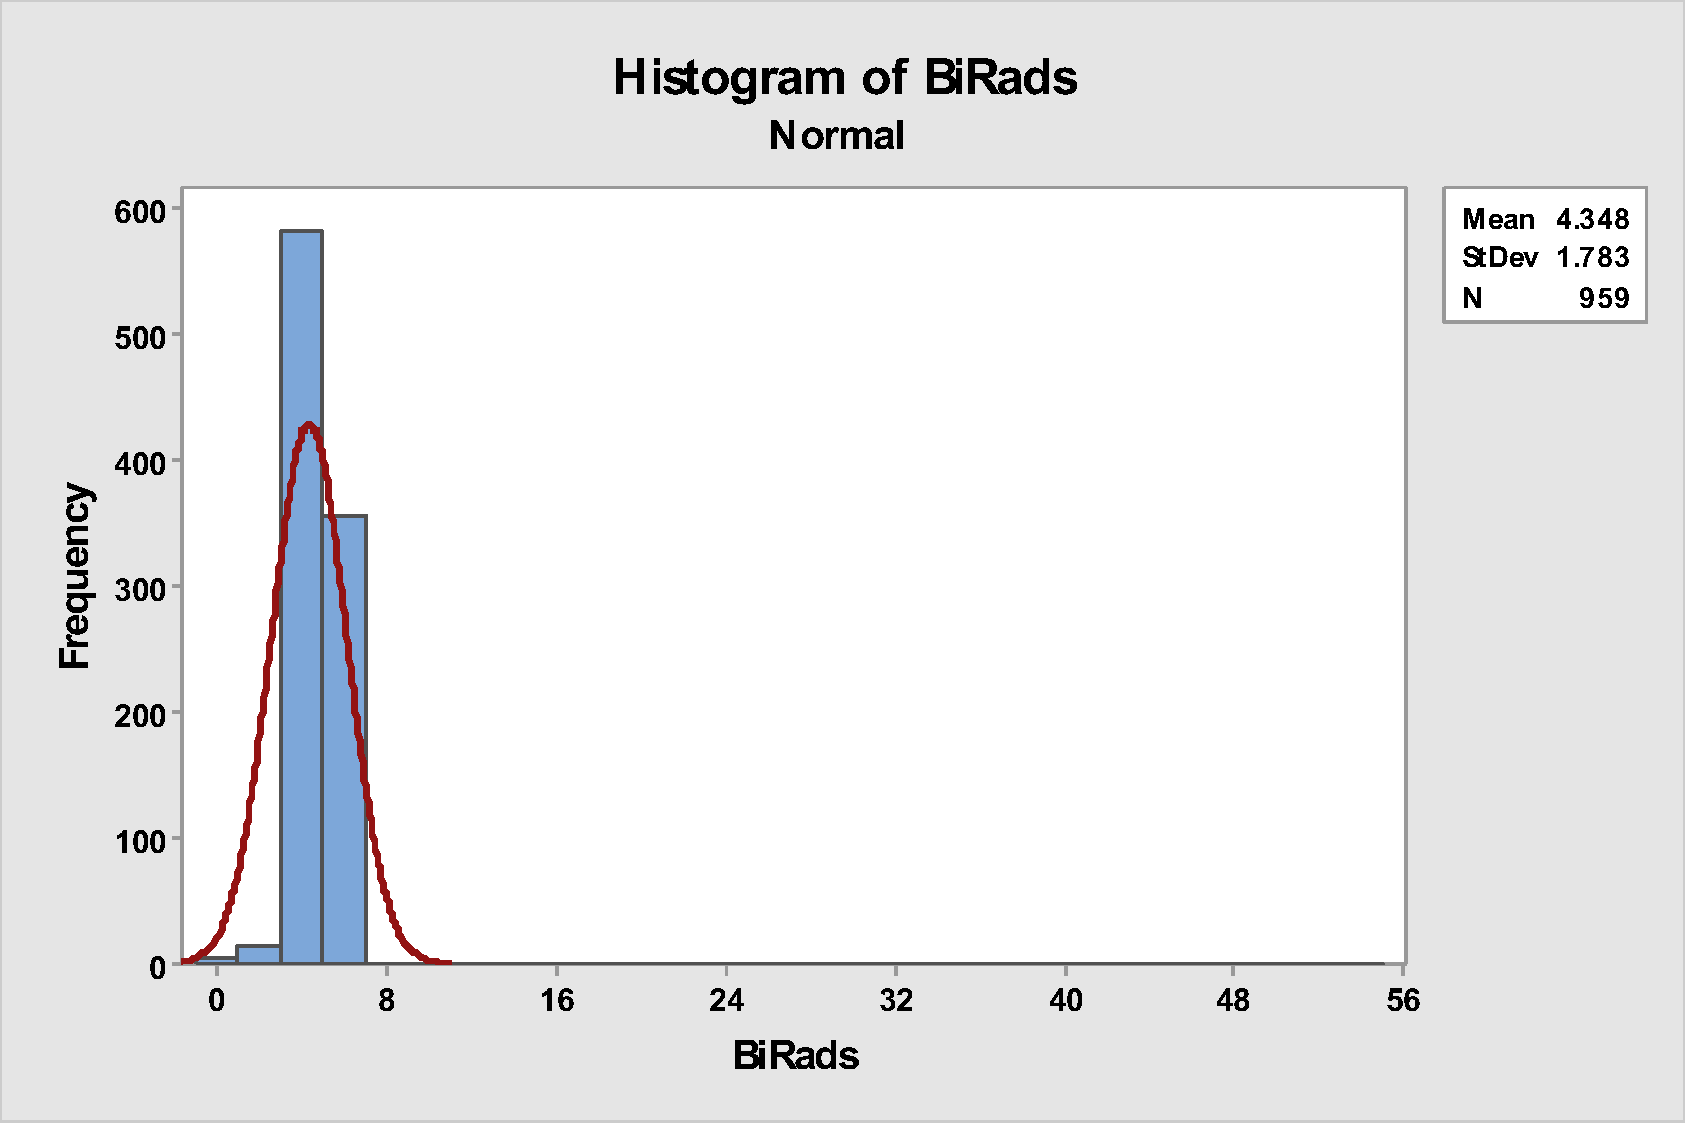
\includegraphics[width=\textwidth]{birads-histogram}
            \caption{Initial}
            \label{fig:birads-histogram}
          \end{subfigure}
          \hfill
          \begin{subfigure}[b]{0.45\textwidth}
            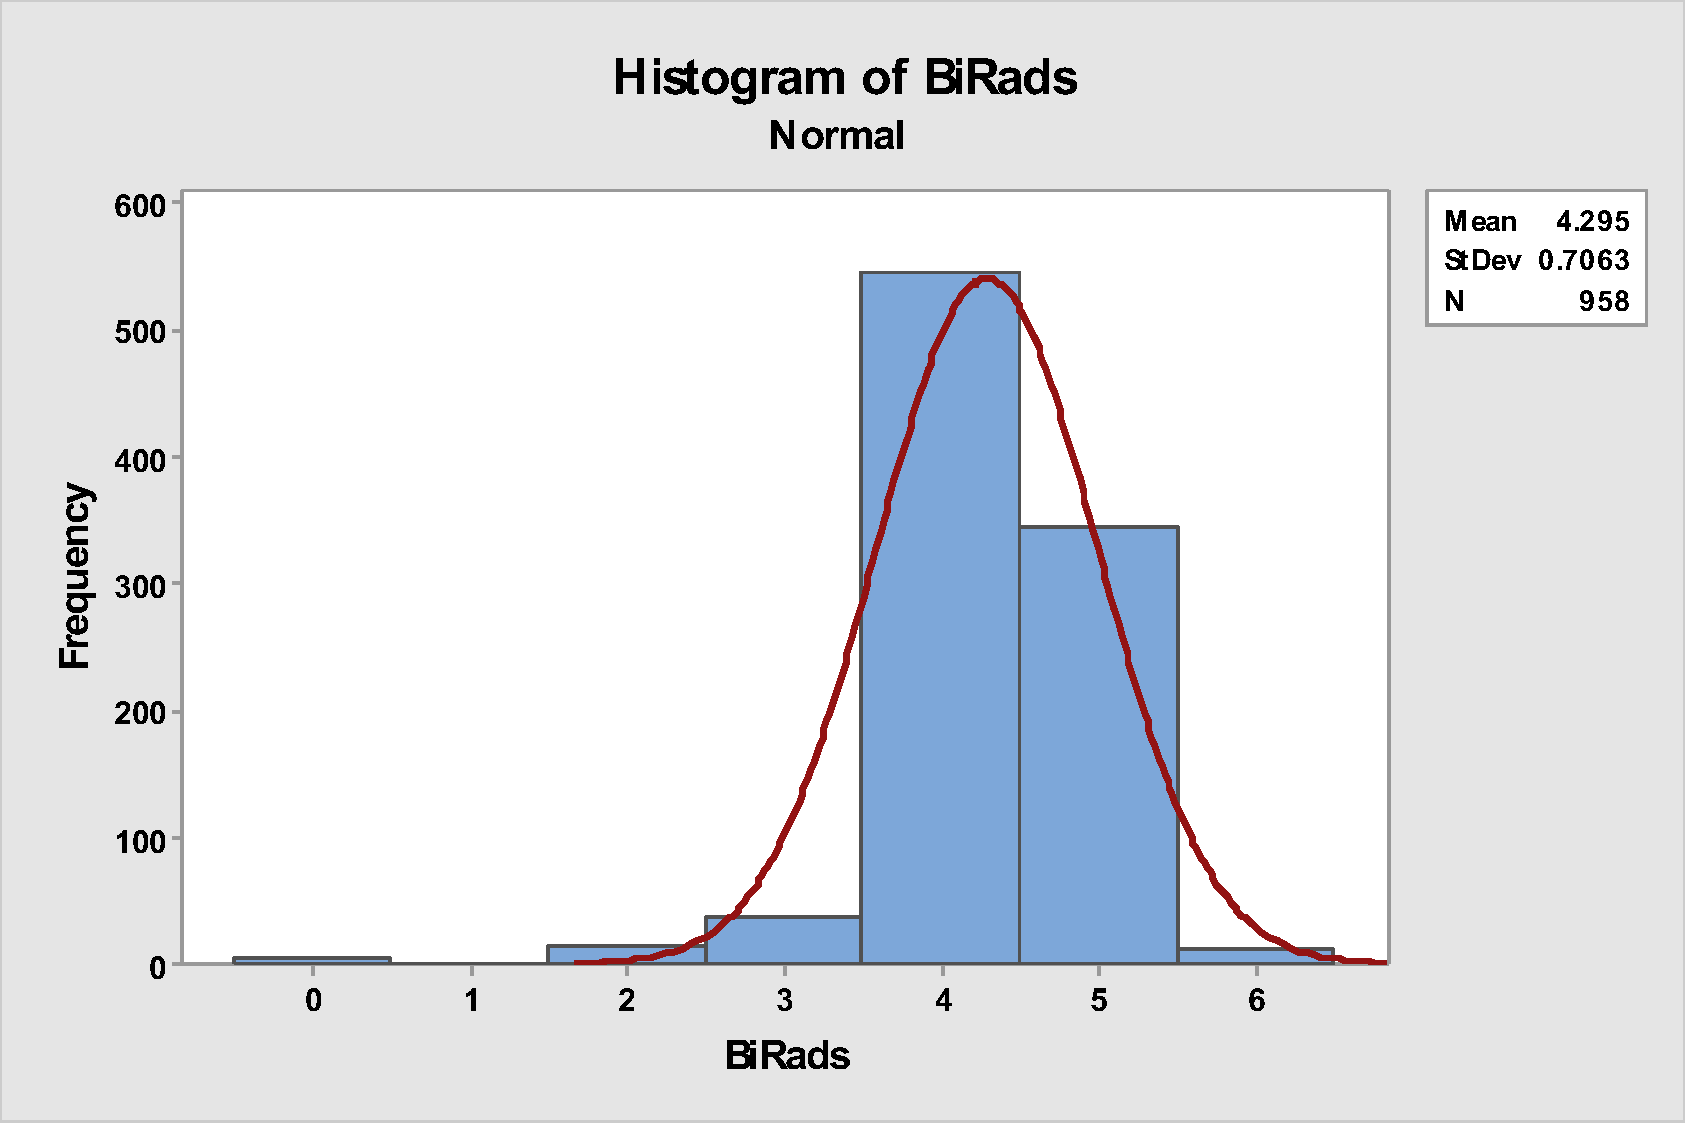
\includegraphics[width=\textwidth]{birads-histogram-no55}
            \caption{Outlier replaced with median}
            \label{fig:birads-histogram-no55}
          \end{subfigure}
          \caption{BI-RADS histogram}
          \label{fig:birads-both-histogram}
        \end{figure}

      \subsubsection{Outliers} \label{birad-outlier}
        Within the BI-RADS attribute there is at least one major outlier as shown in figure \ref{fig:birads-outlier}. This outlier value is ‘55’ and while it could be guessed that this is due to human error of entering a score of ‘5‘ twice accidentally, this outlier must be replaced by the central tendancy. This outlier plot has been repeated in figure \ref{fig:birads-outilier-no55}, with the outlier replaced with the median so as to get a clearer indication of other outliers.

        Figure \ref{fig:birads-outilier-no55} shows that there are several instances with BI-RADS scores of both ‘0’ and ‘6’ which do not exist in the scale. These scores do exist in edition 4 of the BI-RADS scale \citep{d2003breast} however the data descriptors provided with the dataset make no mention of these categories or which edition of the BI-RADS scale it refers to.

        \begin{figure}[H]
          \begin{subfigure}[b]{0.45\textwidth}
            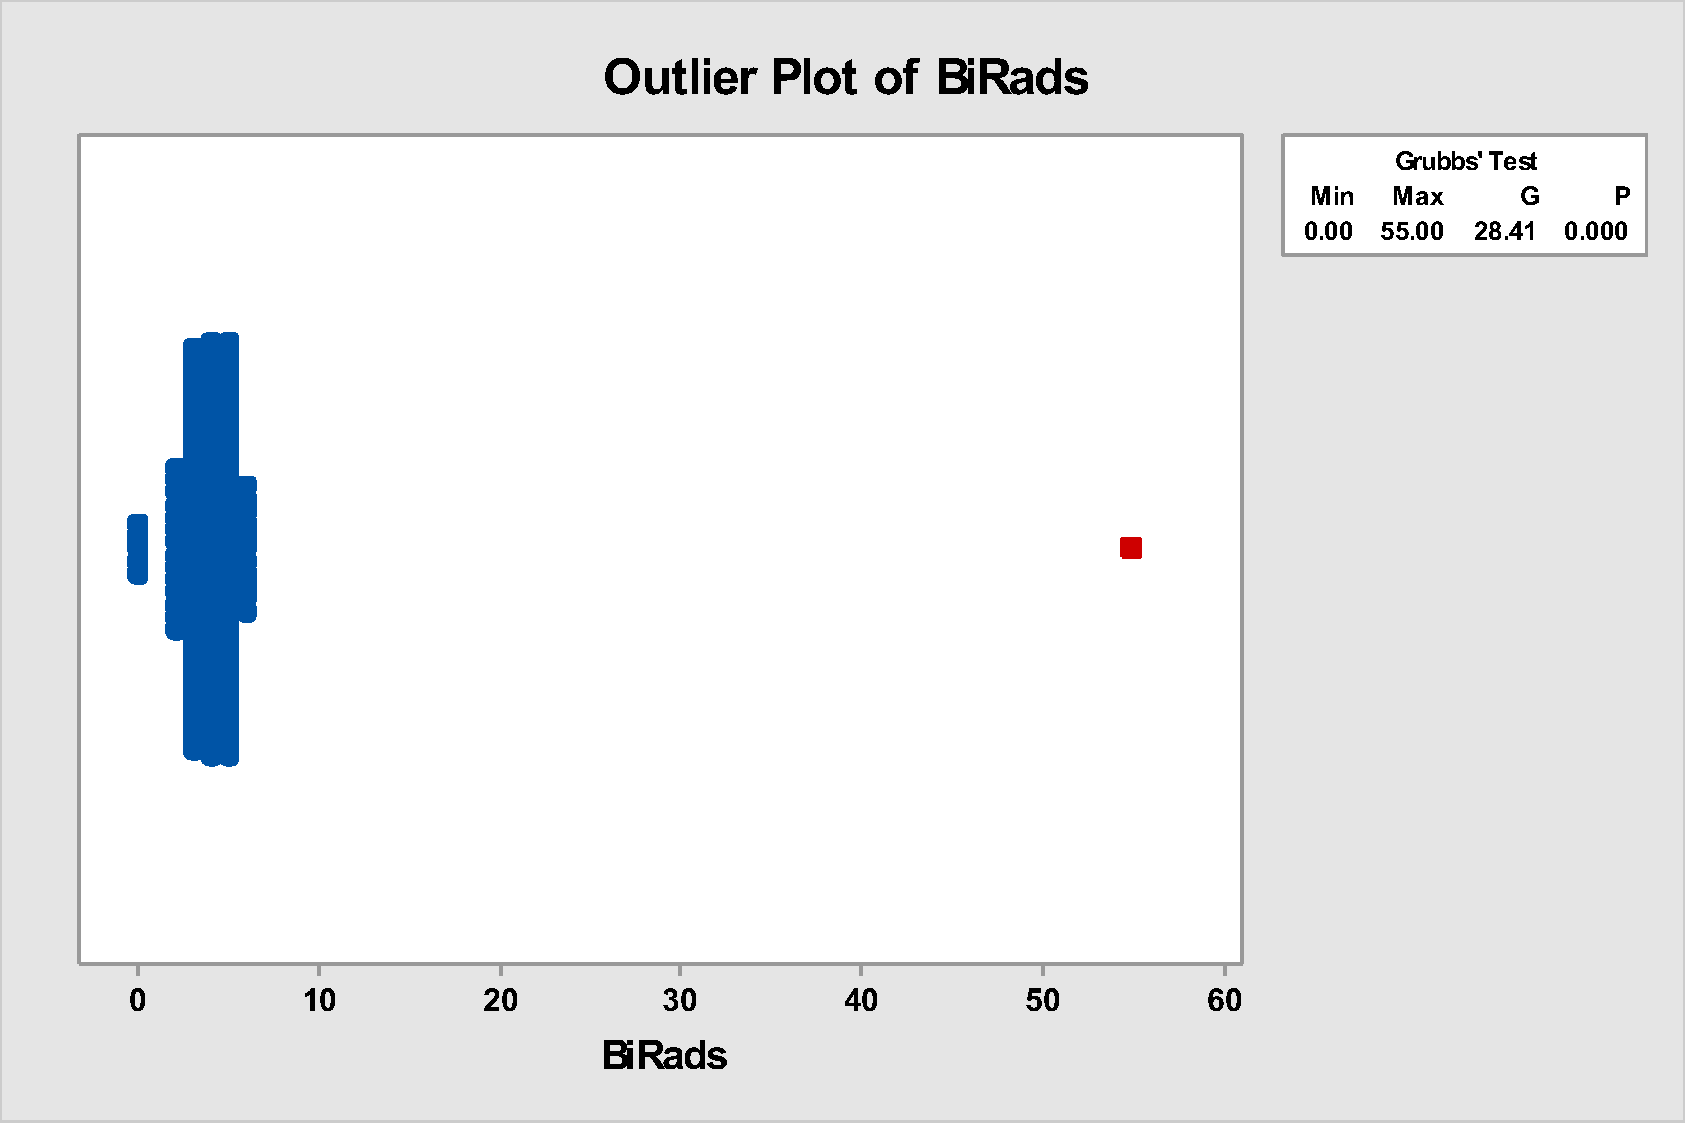
\includegraphics[width=\textwidth]{birads-outlier-plot}
            \caption{Initial}
            \label{fig:birads-outlier}
          \end{subfigure}
          \hfill
          \begin{subfigure}[b]{0.45\textwidth}
            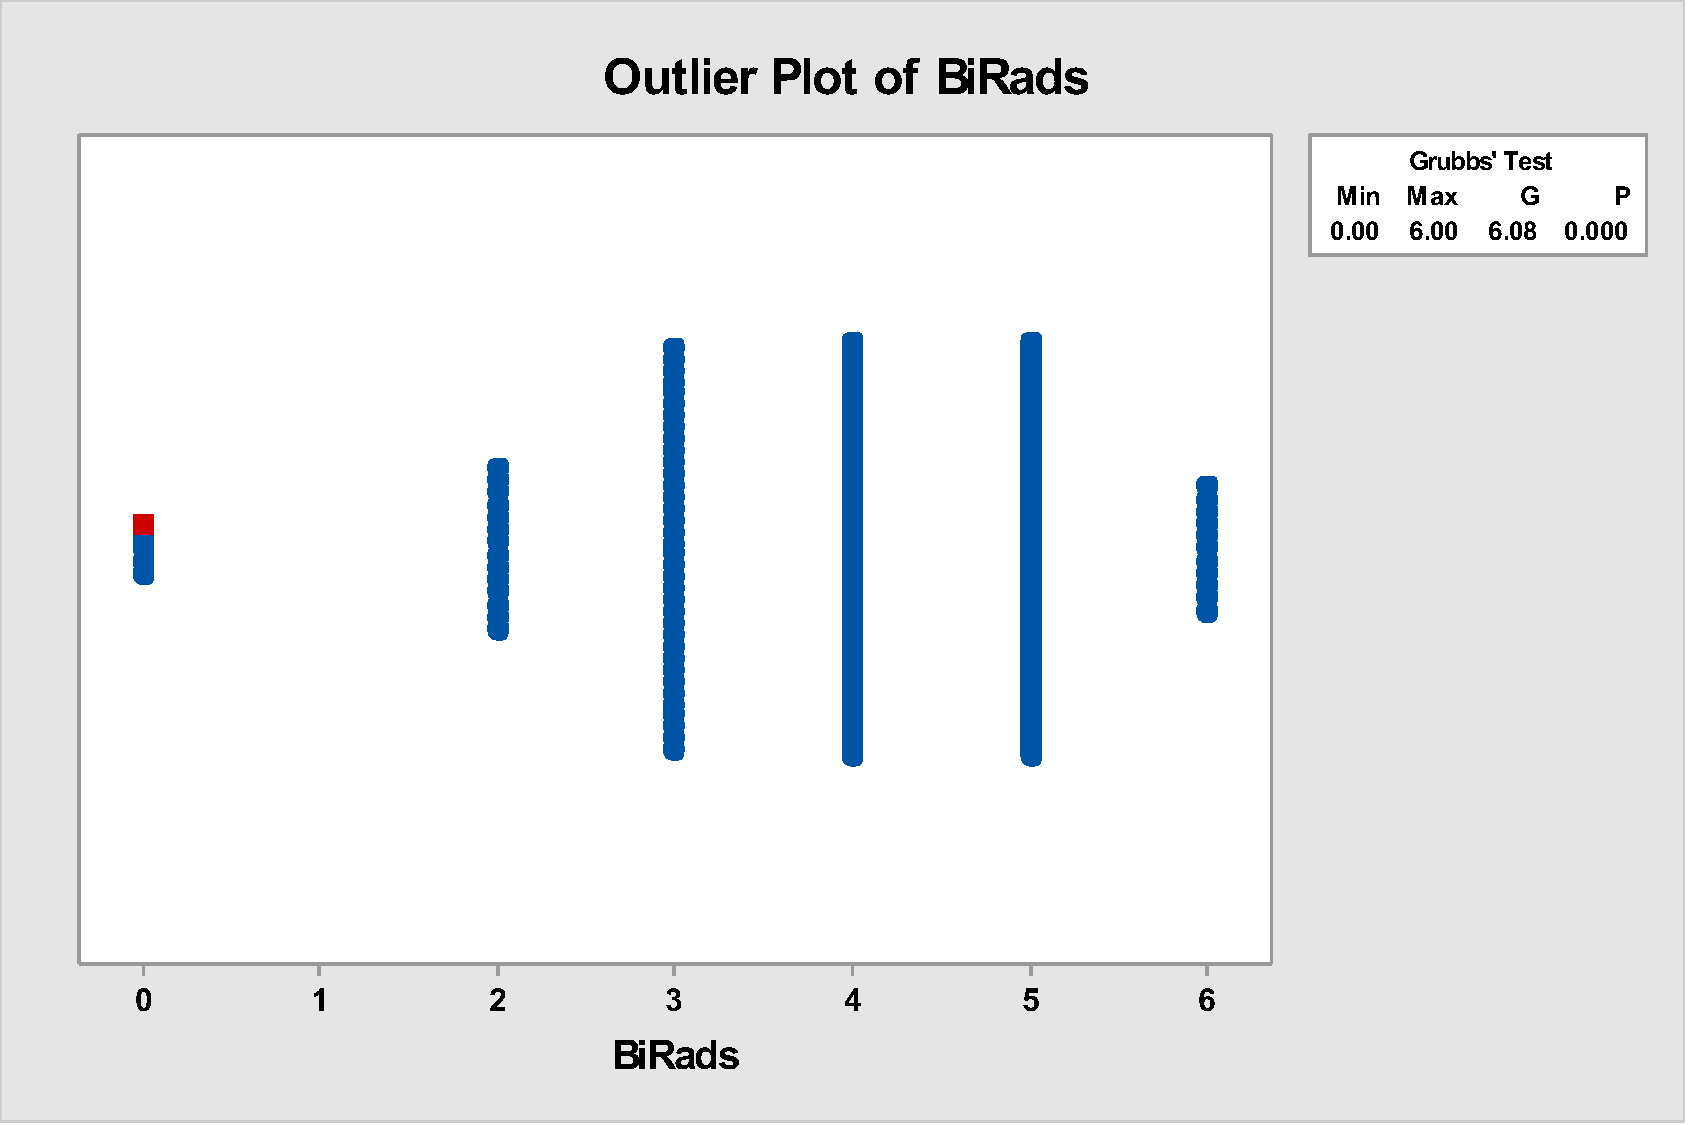
\includegraphics[width=\textwidth]{birads-outlier-plot-no55}
            \caption{Outlier replaced with median}
            \label{fig:birads-outilier-no55}
          \end{subfigure}
          \caption{BI-RADS outlier plots}
        \end{figure}

      \subsubsection{Predictive}
        With the BI-RADS score being a predictive scale, this would mean that if the score of BI-RADS was high then the chance of that instance having a melignant severity would be much higher. This can be shown in figure \ref{fig:birads-severity-correlation} where it is shown that there is a slight correlation between a higher BI-RADS score and \% of severity classification.

        \begin{figure}[H]
          \centering
          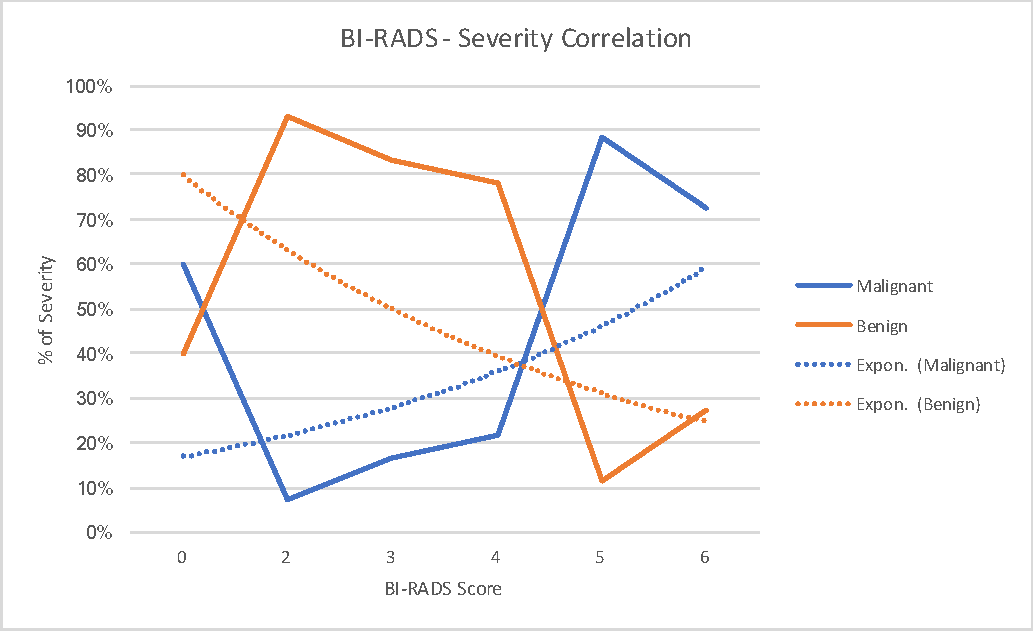
\includegraphics[width=0.6\textwidth]{birads-severity-correlation}
          \caption{BI-RADS - Severity correlation}
          \label{fig:birads-severity-correlation}
        \end{figure}

        \begin{figure}[H]
          \begin{subfigure}[b]{0.45\textwidth}
            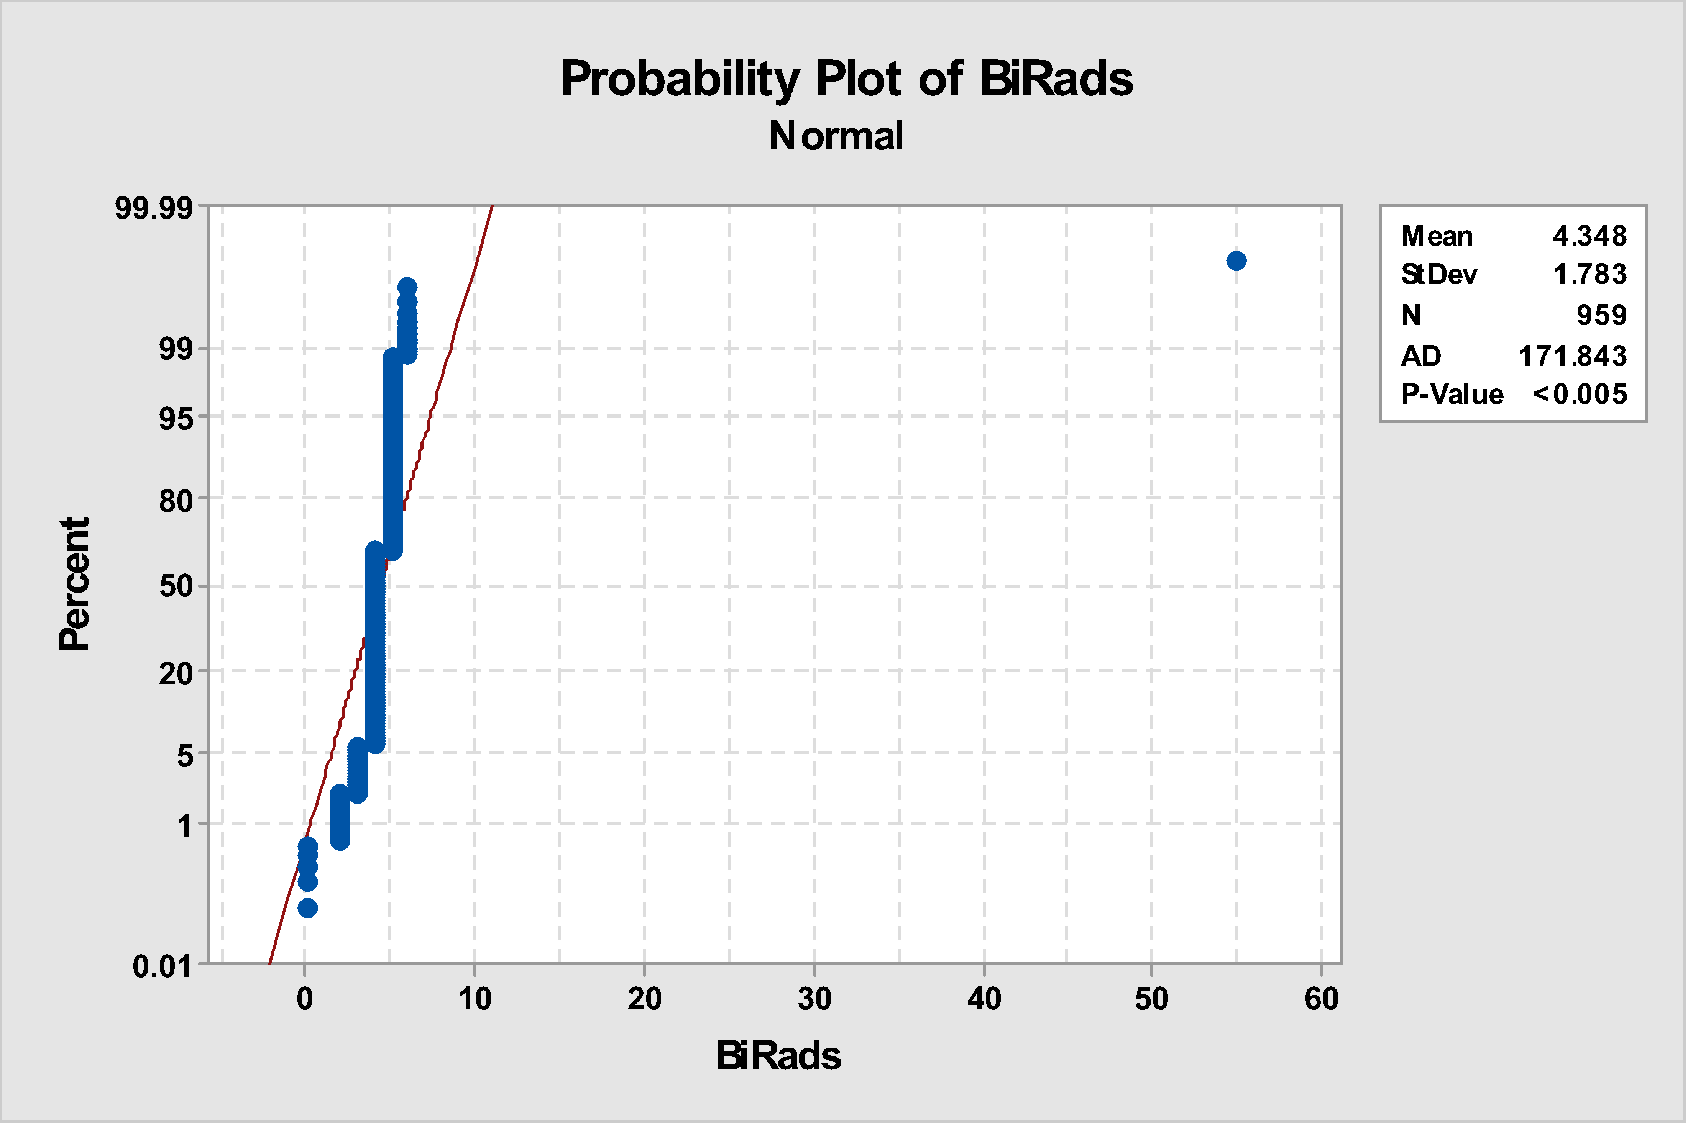
\includegraphics[width=\textwidth]{birads-probability}
            \caption{Initial}
            \label{fig:birads-probability}
          \end{subfigure}
          \hfill
          \begin{subfigure}[b]{0.45\textwidth}
            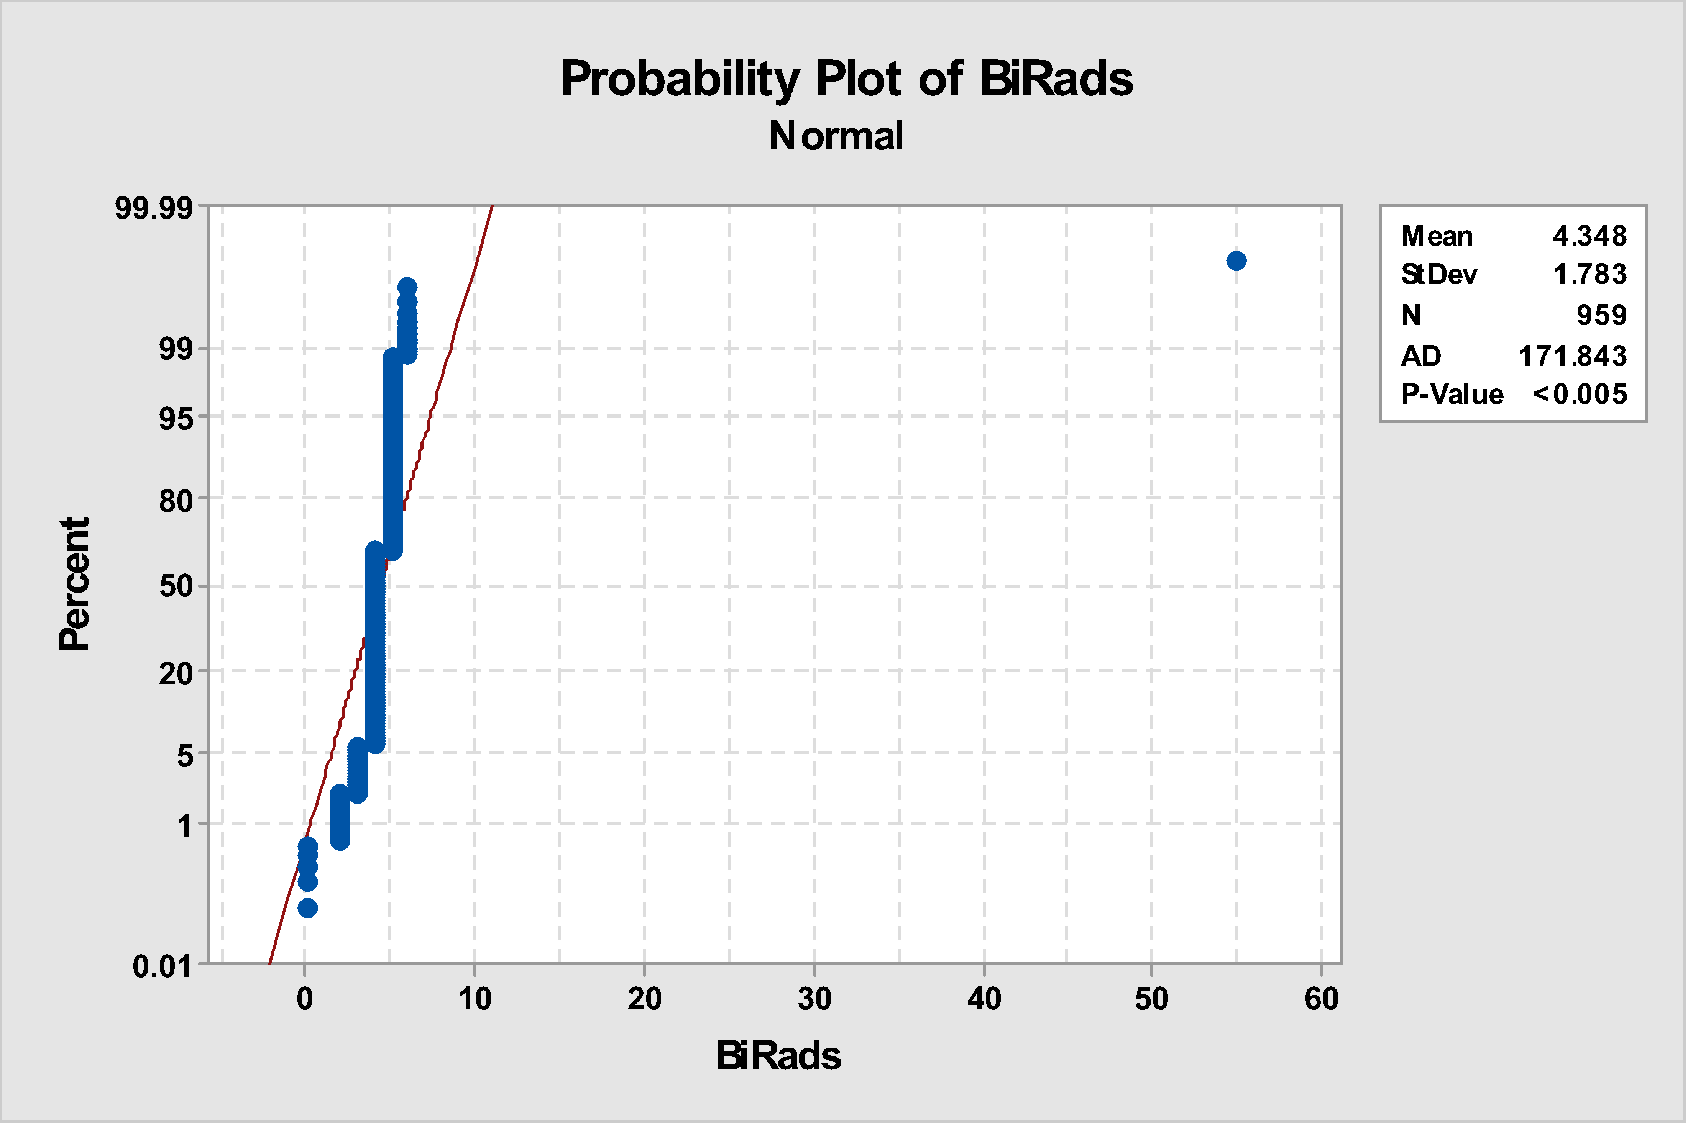
\includegraphics[width=\textwidth]{birads-probability}
            \caption{Outlier replaced with median}
            \label{fig:birads-probability}
          \end{subfigure}
          \caption{BI-RADS probability.}
        \end{figure}

    \subsection{Age}
      \subsubsection{Measurement}
        This is the only non-predictive attribute provided in the dataset, and is a simple ratio scale of the patients age.

      \subsubsection{Distribution}
        As shown in figure \ref{fig:age-histogram}, the distribution of age within the dataset is non-normal and is skewed very slightly to the right.

        \begin{figure}[H]
          \centering
          \begin{minipage}[b]{0.45\textwidth}
            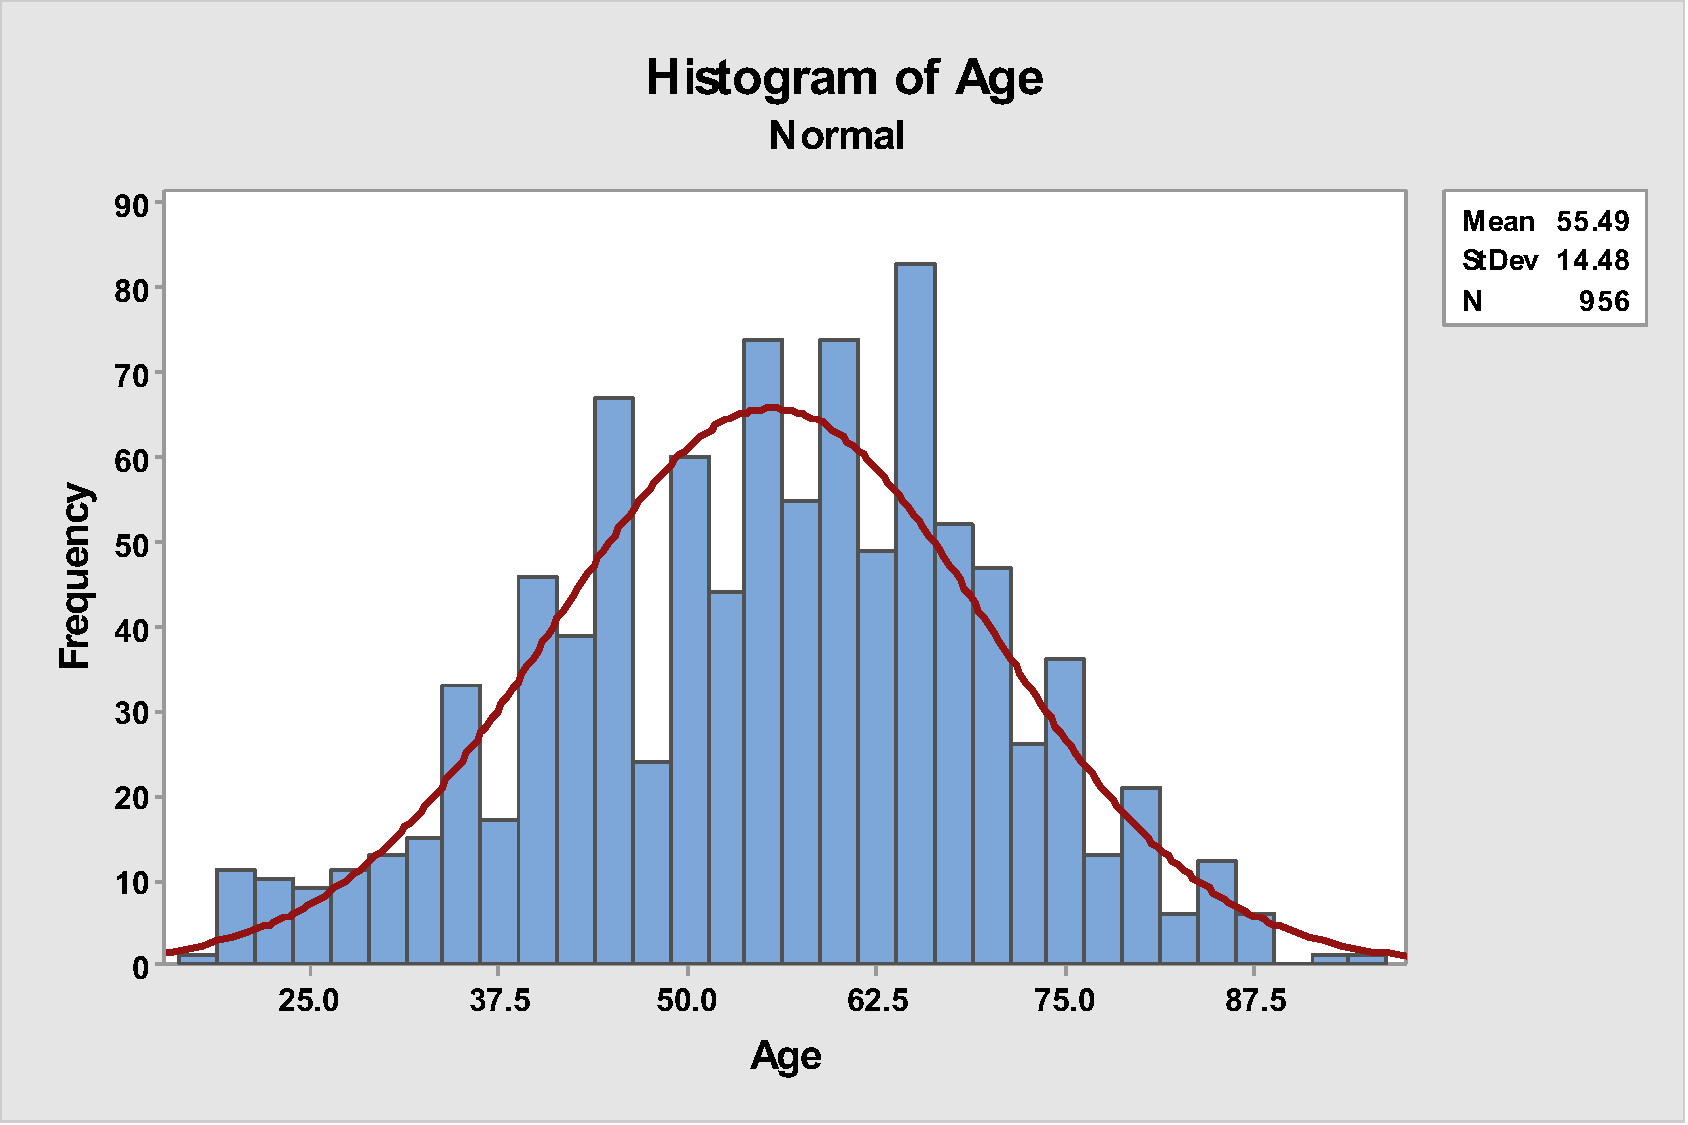
\includegraphics[width=\textwidth]{age-histogram}
            \caption{Age histogram}
            \label{fig:age-histogram}
          \end{minipage}
          \hfill
          \begin{minipage}[b]{0.45\textwidth}
            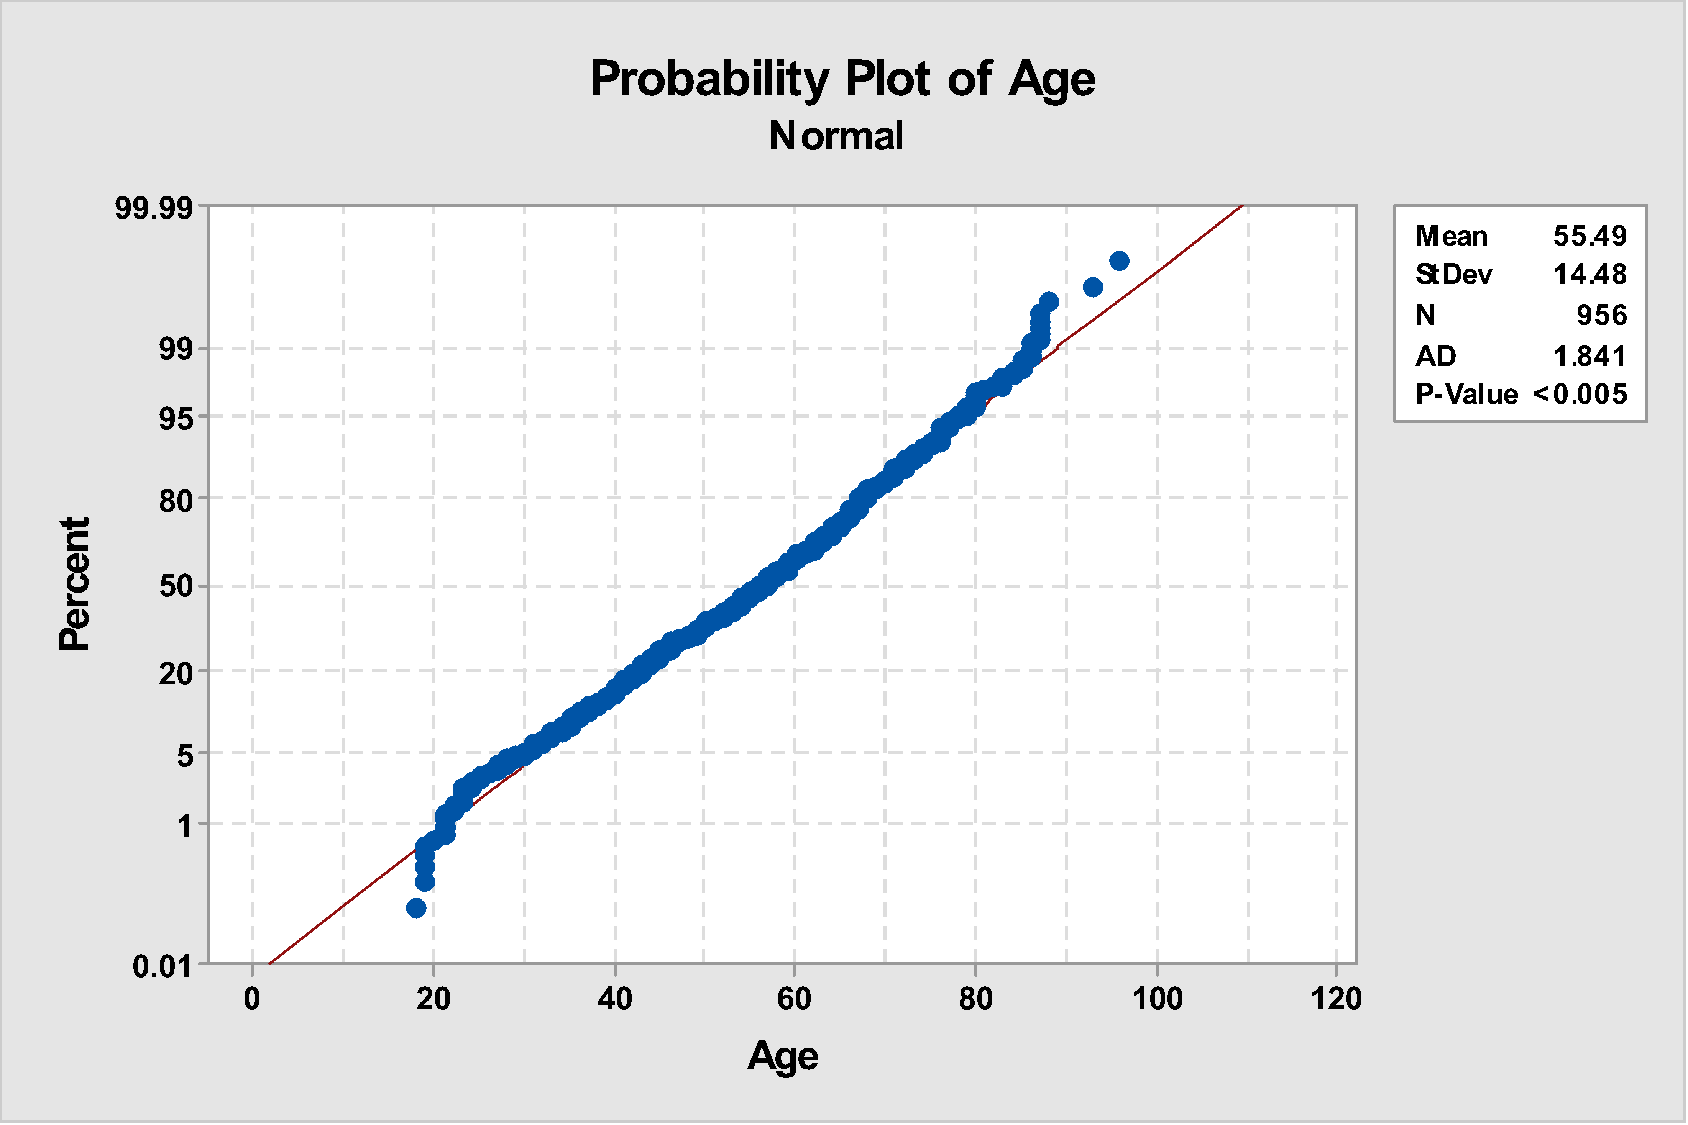
\includegraphics[width=\textwidth]{age-probability}
            \caption{Age probability}
            \label{fig:age-probability}
          \end{minipage}
        \end{figure}

      \subsubsection{Outliers}
        There does not appear to be any outliers in the age attribute as shown by figure \ref{fig:age-outlier-plot}. There are, however, 2 missing values within the attribute. The central tendancy for this attribute should be the median due to the fact that the scale type is ratio and that the distribution is non-normal.

        \begin{figure}[H]
          \centering
          \begin{minipage}[b]{0.45\textwidth}
            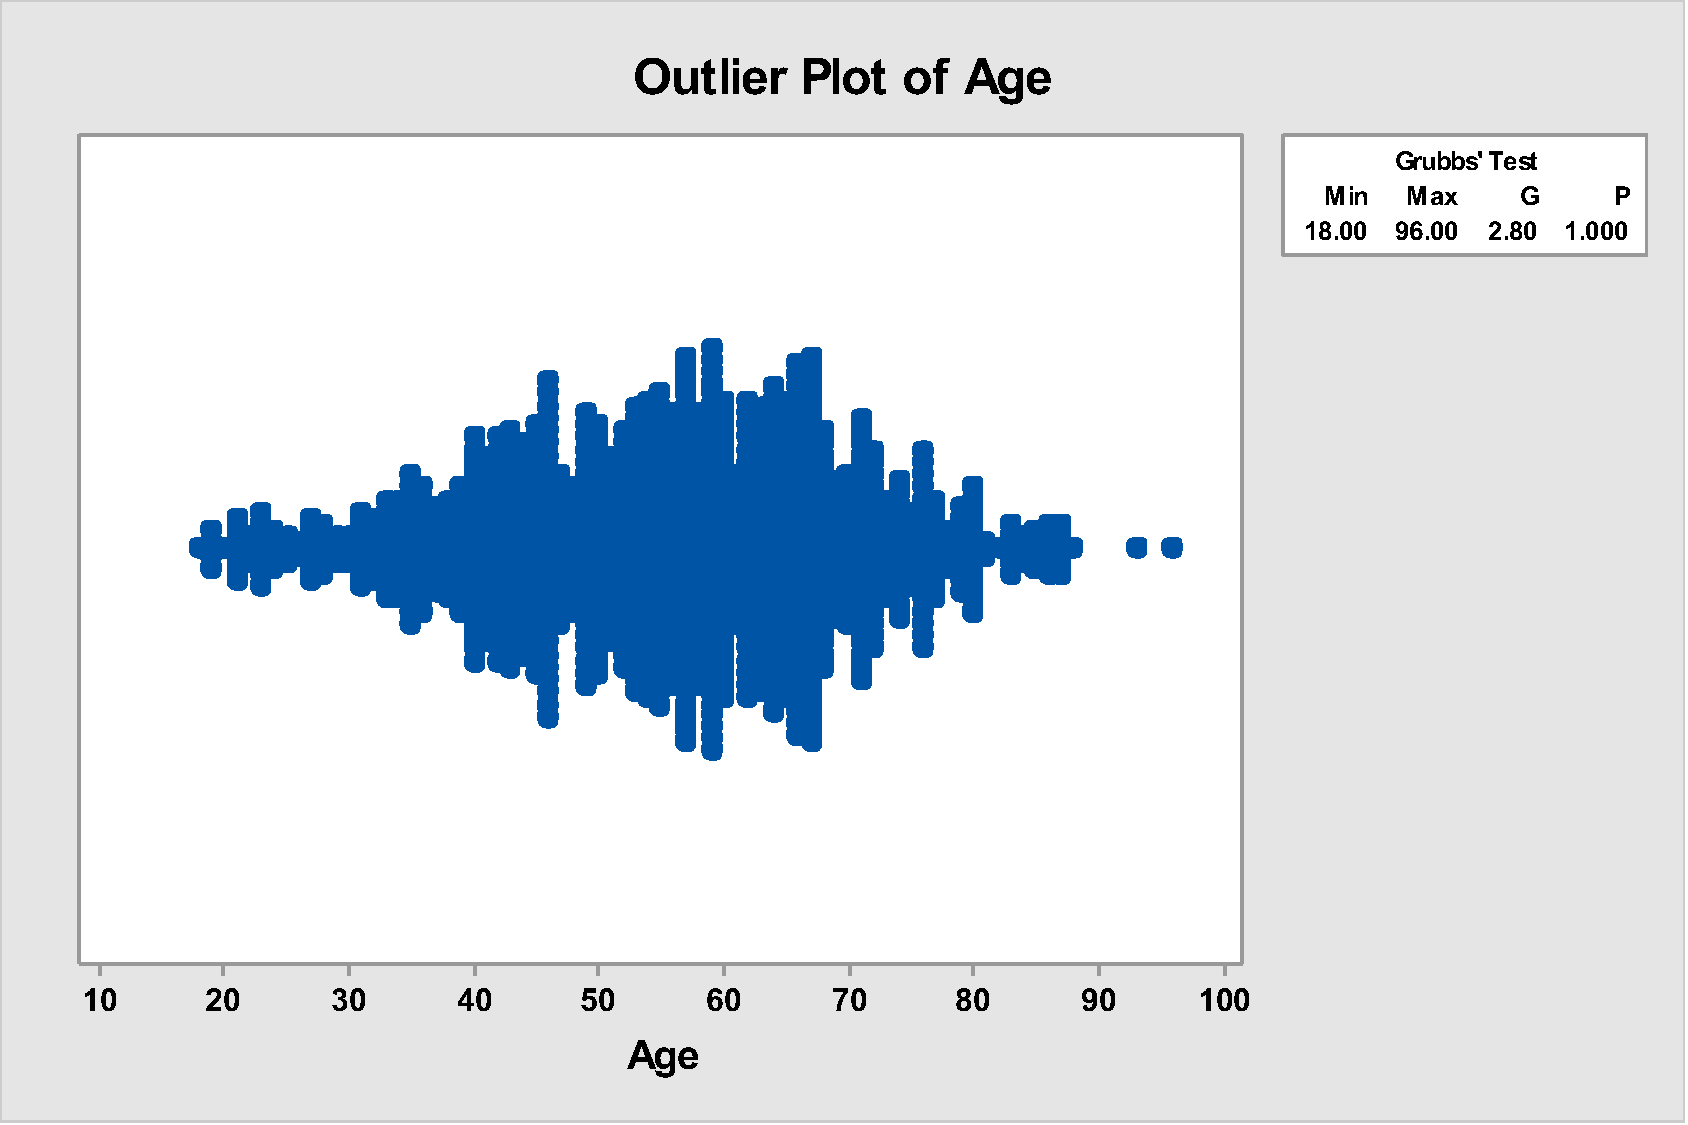
\includegraphics[width=\textwidth]{age-outlier-plot}
            \caption{Age outlier plot}
            \label{fig:age-outlier-plot}
          \end{minipage}
          \hfill
          \begin{minipage}[b]{0.45\textwidth}
            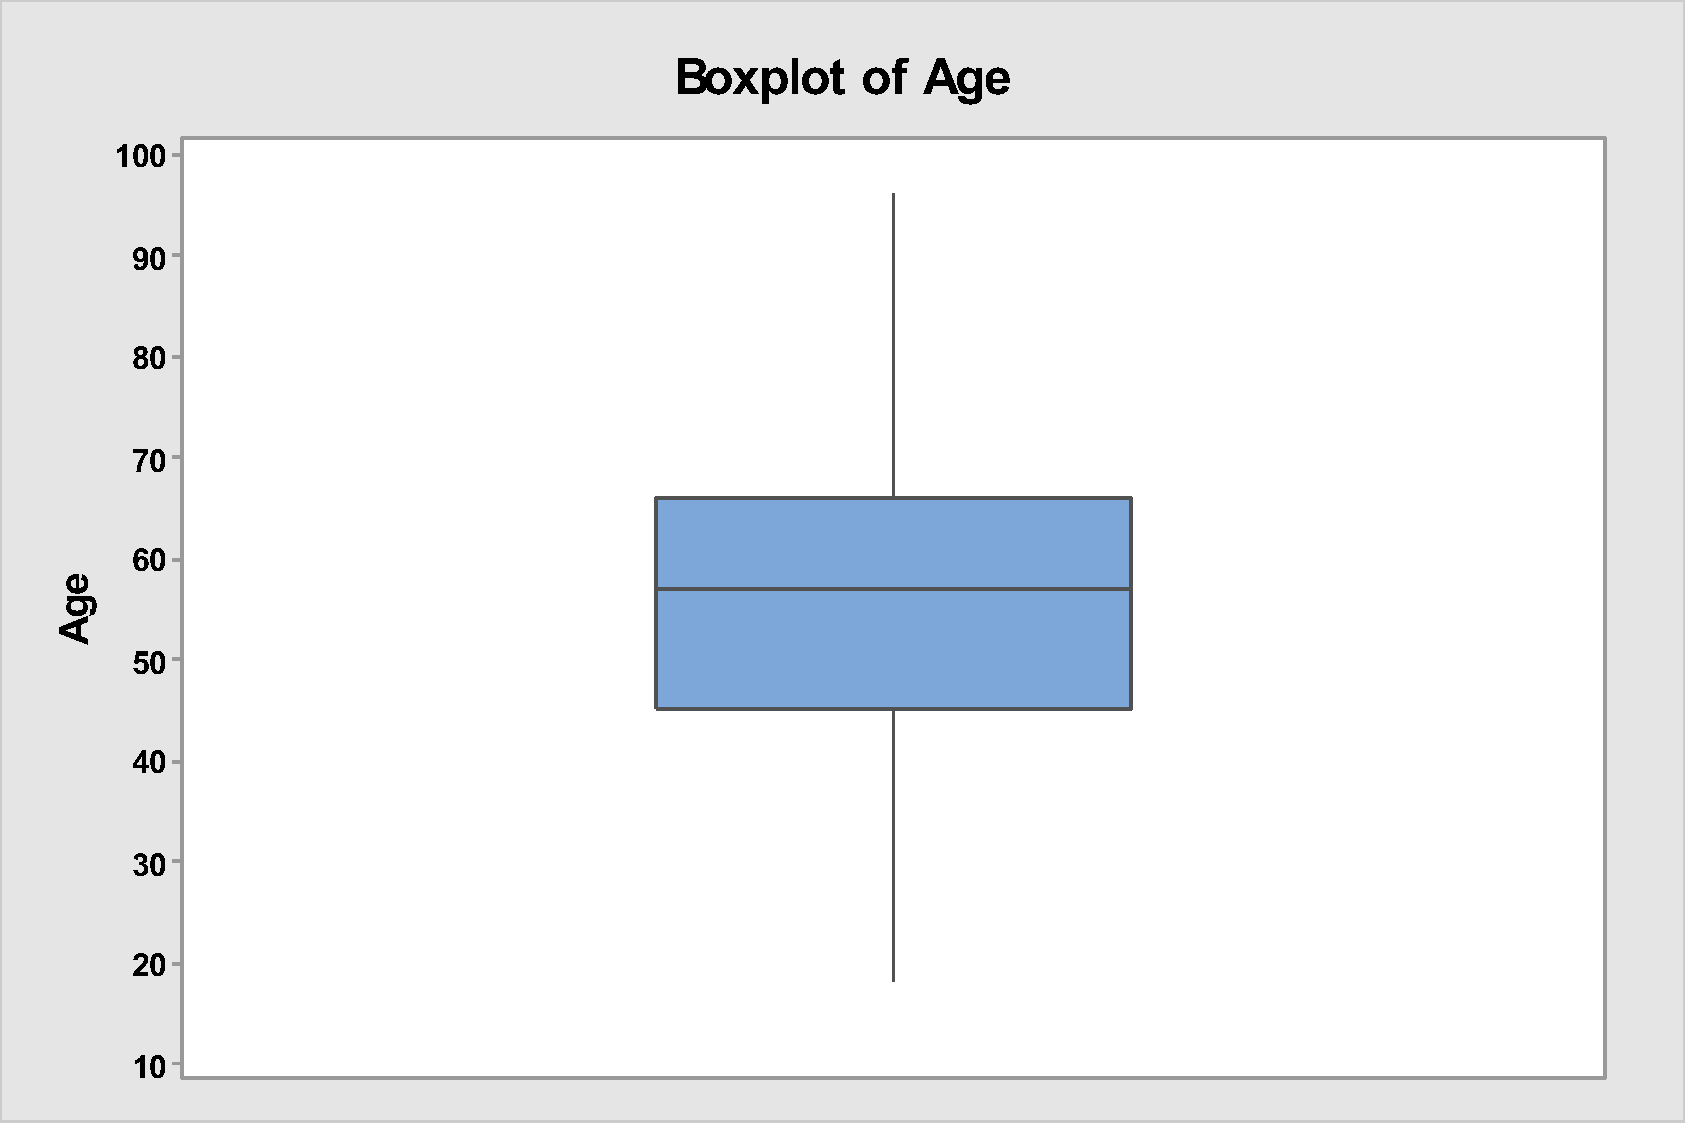
\includegraphics[width=\textwidth]{age-boxplot}
            \caption{Age boxplot}
            \label{fig:age-boxplot}
          \end{minipage}
        \end{figure}

      \subsubsection{Predictive}
        While age itself is not a predictive attribute, it has been shown that women diagnosed with breast cancer are much more likely to be above 50 years of age \citep{kerlikowske1993mammography}. This can be backed up by figure \ref{fig:age-severity-correlation} which shows a clear correlation between age and the percent of severity classifications per age group in the provided dataset

        Due to this and the findings with the BI-RADS attribute, it could be inferred that those with an age above 50 and a high BI-RADS score have a very high change of having a malignant severity.

        \begin{figure}[H]
          \centering
          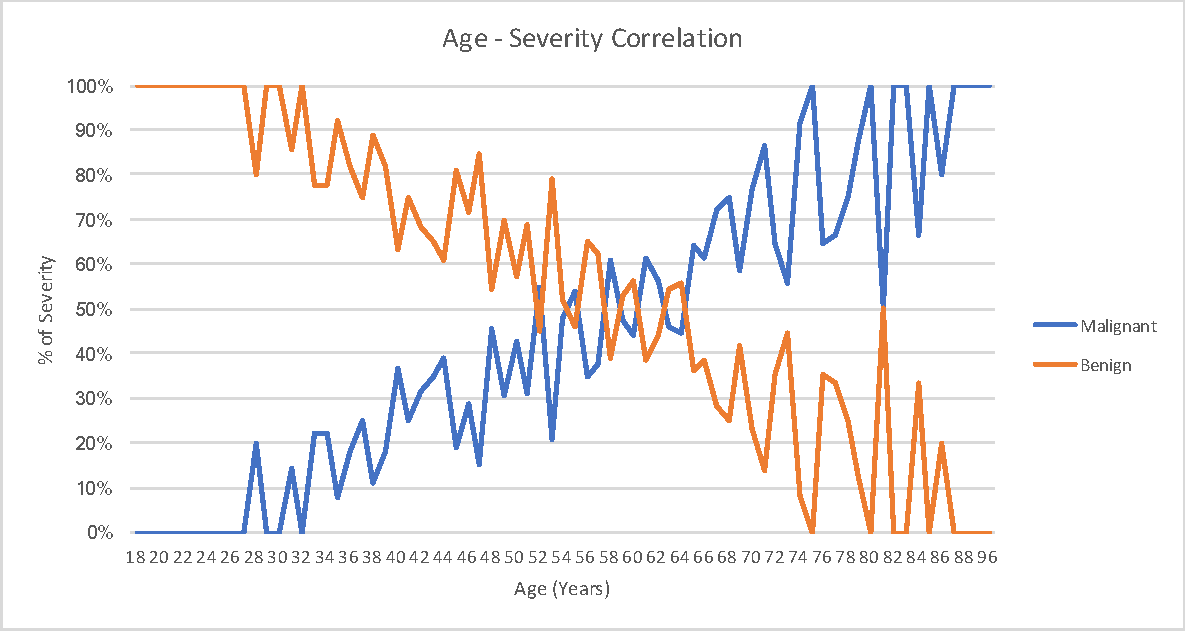
\includegraphics[width=0.6\textwidth]{age-severity-correlation}
          \caption{Age - Severity correlation}
          \label{fig:age-severity-correlation}
        \end{figure}

    \subsection{Shape}
      \subsubsection{Measurement}
        This attribute is used to describe the shape of the mass being investigated. It is a nominal attribute as the number scale has no bearing on its meaning. Below are the definitions for each of the shape scores as defined by the dataset.

        \begin{enumerate}[label=\arabic*)]
          \item Round
          \item Oval
          \item Lobular
          \item Irregular
        \end{enumerate}

        When performing experiments in WEKA, the values in this attribute will be replaced with text values to ensure its processing as a nominal attribute.

      \subsubsection{Distribution}
        As shown in figure \ref{fig:shape-histogram}, the shape attribute is non-normal and is skewed to the right.

        \begin{figure}[H]
          \centering
          \begin{minipage}[b]{0.45\textwidth}
            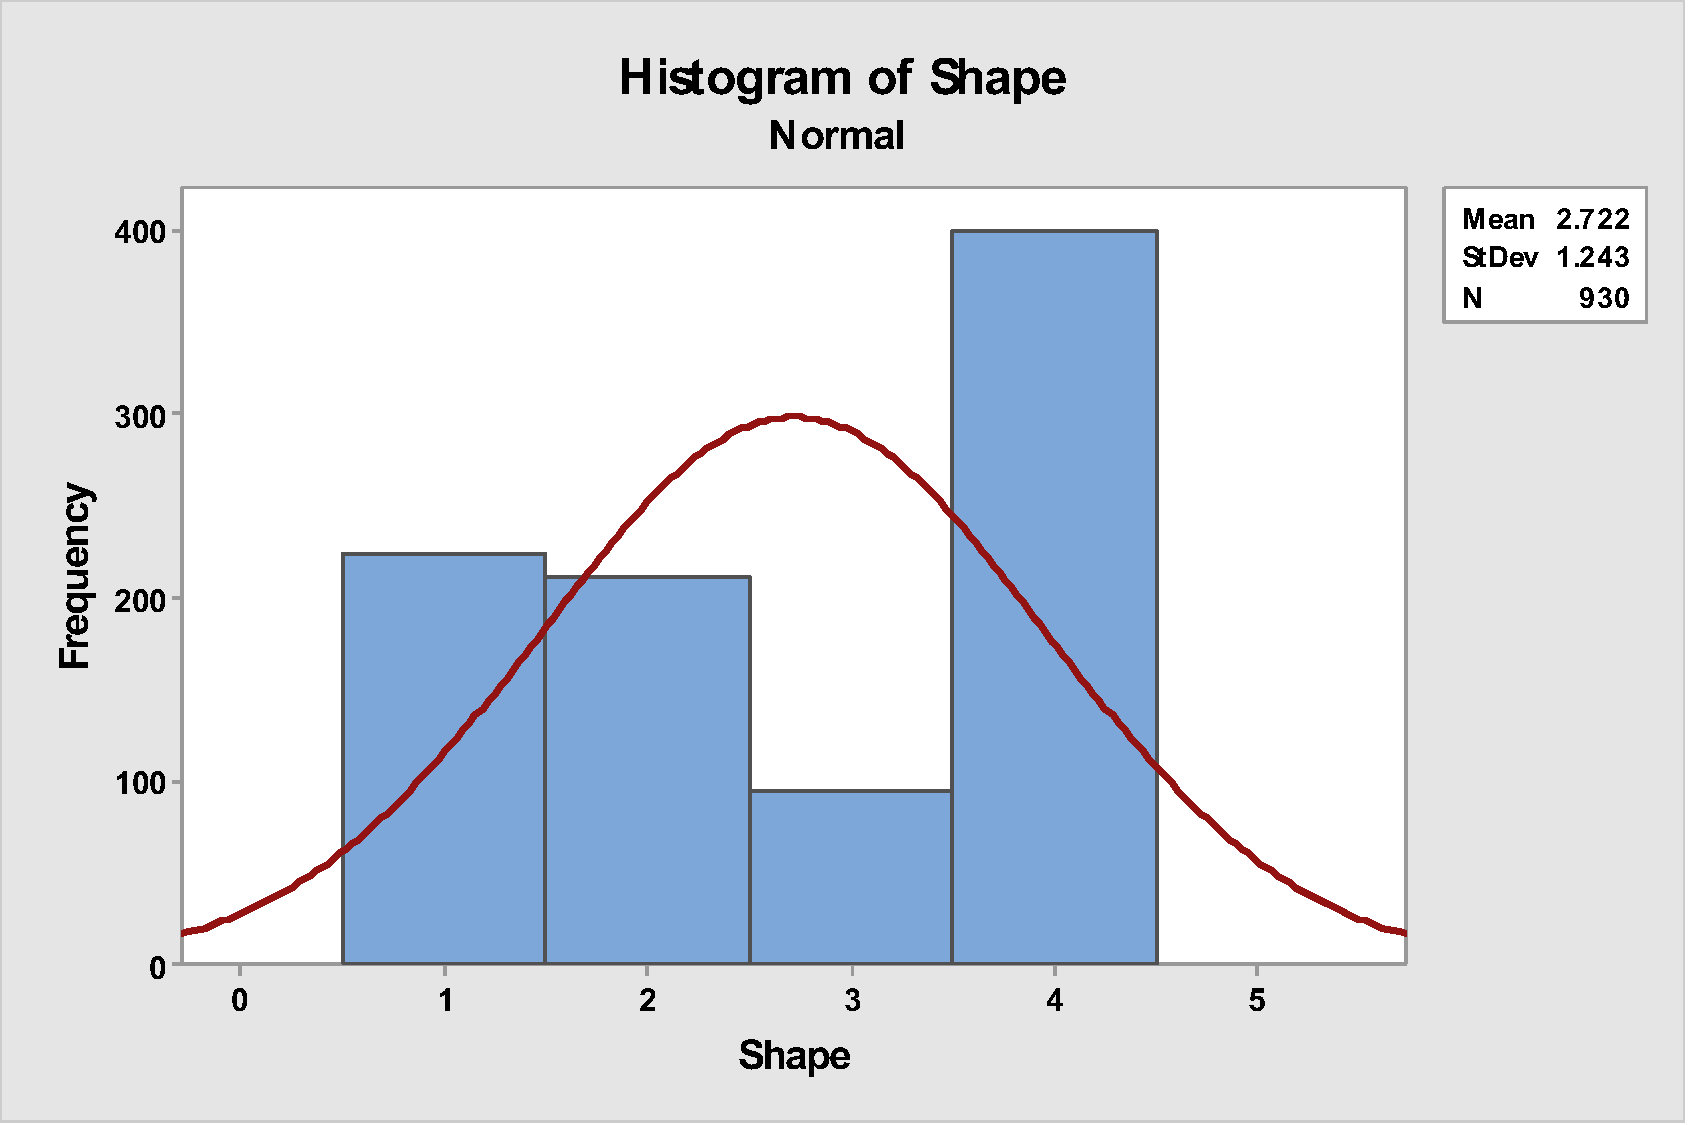
\includegraphics[width=\textwidth]{shape-histogram}
            \caption{Shape histogram}
            \label{fig:shape-histogram}
          \end{minipage}
          \hfill
          \begin{minipage}[b]{0.45\textwidth}
            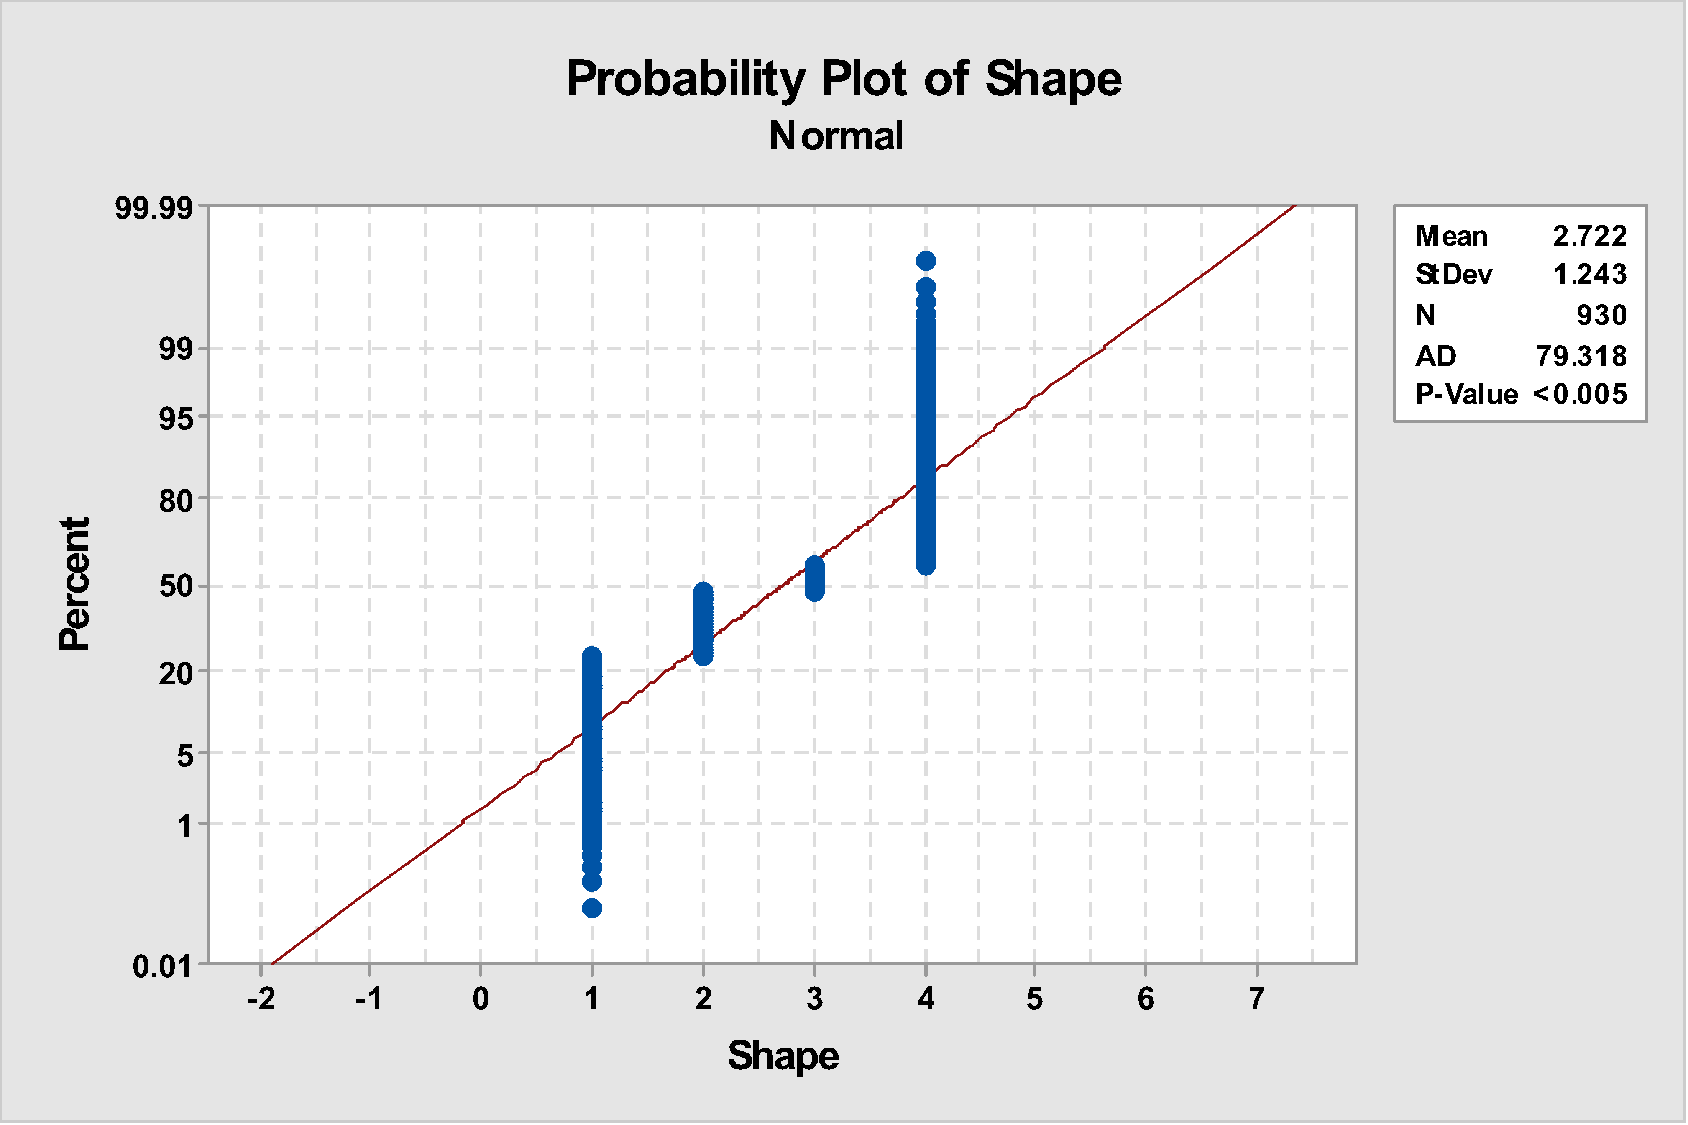
\includegraphics[width=\textwidth]{shape-probability}
            \caption{Shape probability}
            \label{fig:shape-probability}
          \end{minipage}
        \end{figure}

      \subsubsection{Outliers}
        While there do not appear to be any outliers within this attribute, it does contain 31 missing values. Due to it being nominal the central tendancy for these values should be the mode.

      \subsubsection{Predictive}
        In figure \ref{fig:shape-severity-correlation} below it can be seen that while shape is not on an ordinal scale, a higher score of shape is correlated with a higher chance of a malignant severity.

        \begin{figure}[H]
          \centering
          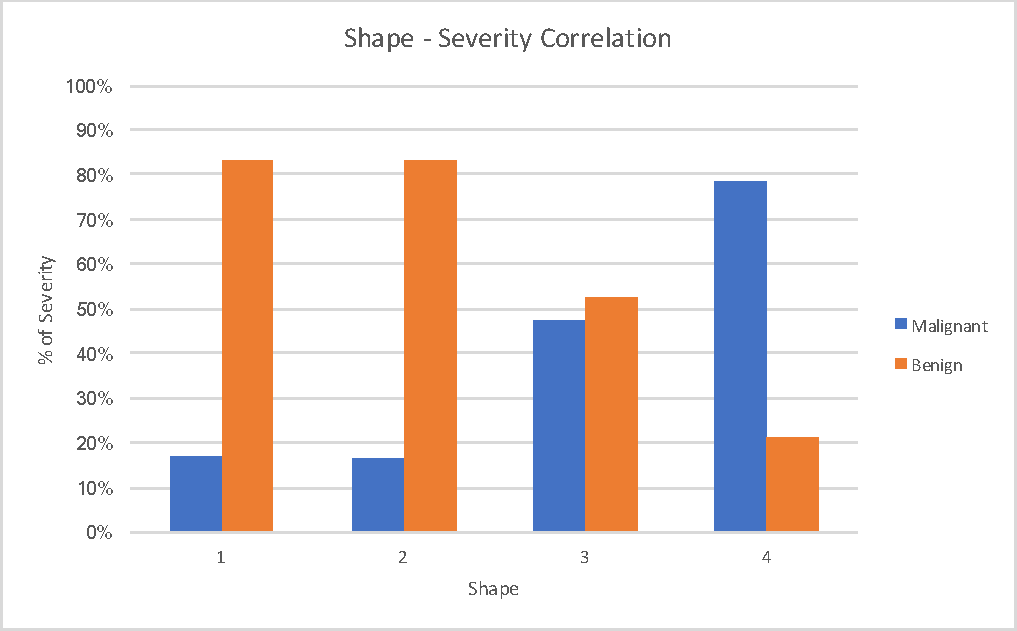
\includegraphics[width=0.6\textwidth]{shape-severity-correlation}
          \caption{Shape - Severity correlation}
          \label{fig:shape-severity-correlation}
        \end{figure}

    \subsection{Margin}
      \subsubsection{Measurement}
        The margin attribute is used to describe the edges of the mass and their distinctiveness from the rest of the breast tissue within the scan. This is also a nominal attribute as there is no scale for the margin descriptors. Below are the 5 different definitions for each of the margin scores.

        \begin{enumerate}[label=\arabic*)]
          \item Circumscribed
          \item Microlobulated
          \item Obscured
          \item Ill-defined
          \item Spiculated
        \end{enumerate}

        As with the previous attribute, when performing experiments in WEKA the values in this attribute will be replaced with text values to ensure its processing as a nominal attribute.

      \subsubsection{Distribution}
        The distribution of values in the margin attribute appears to be non-normal and is skewed to the right.

        \begin{figure}[H]
          \centering
          \begin{minipage}[b]{0.45\textwidth}
            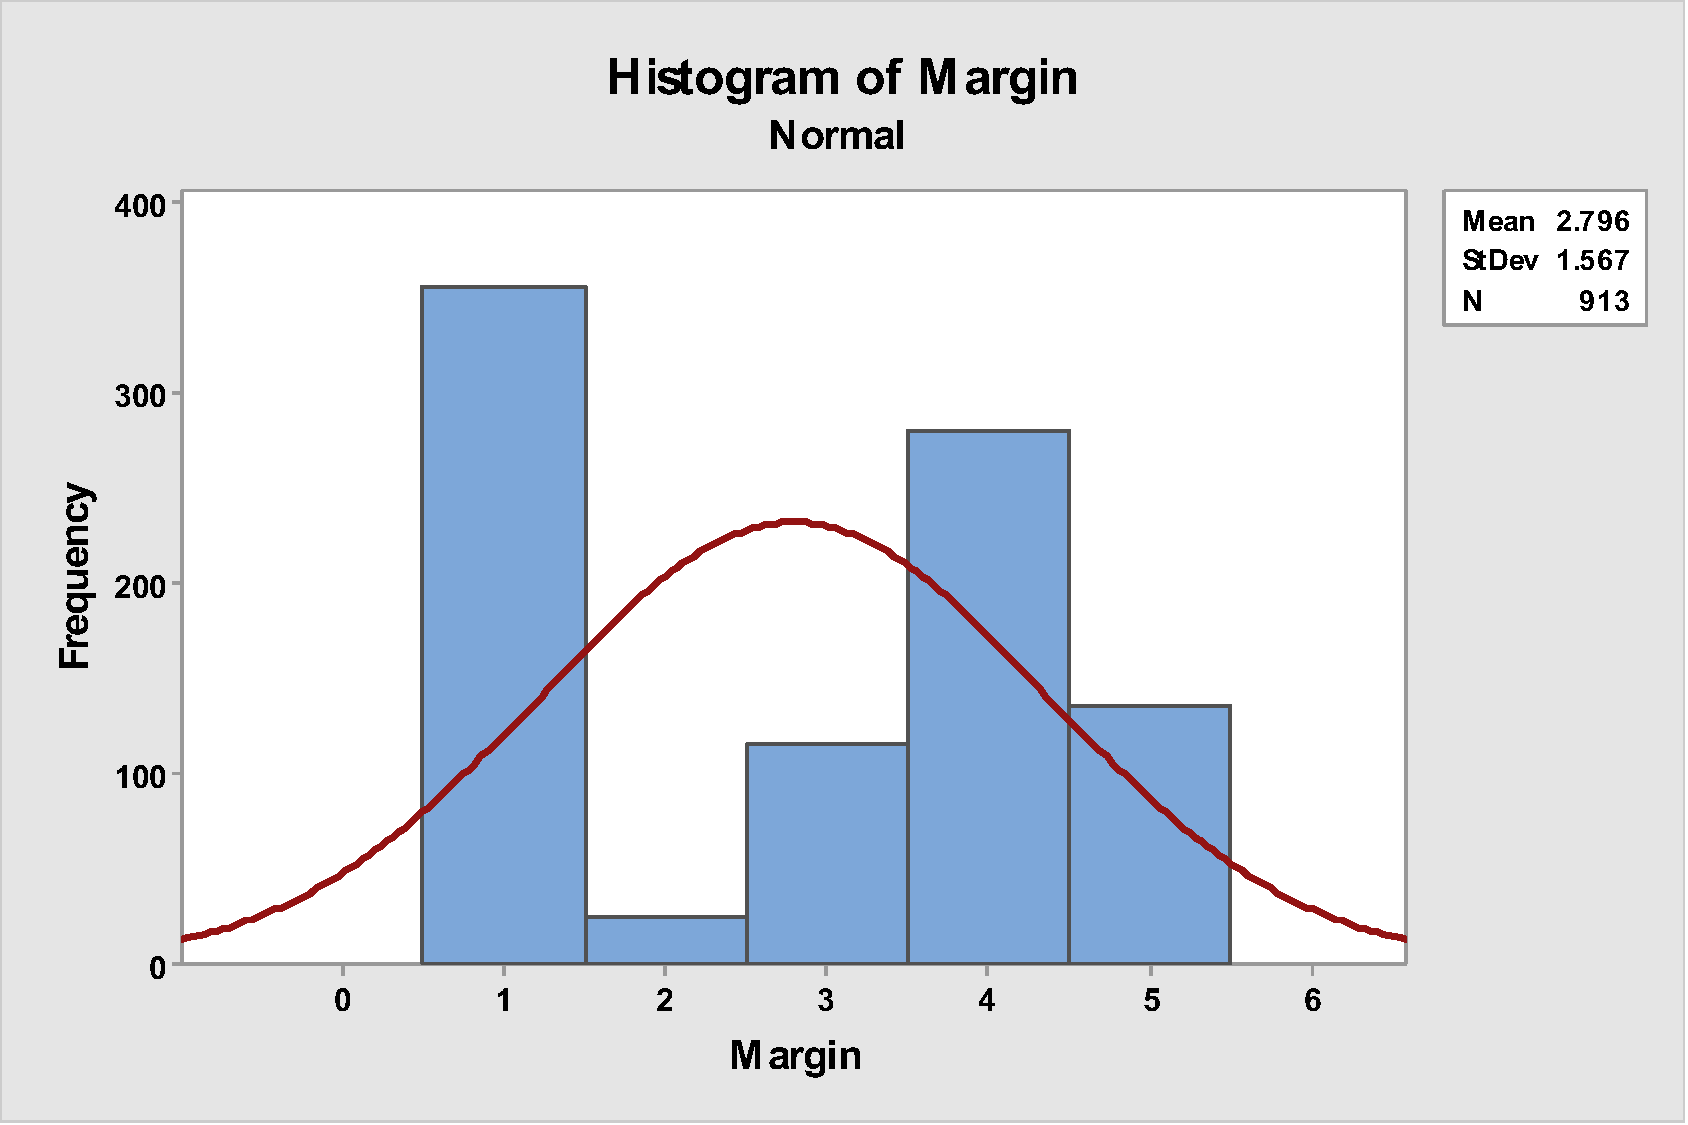
\includegraphics[width=\textwidth]{margin-histogram}
            \caption{Margin histogram}
            \label{fig:margin-histogram}
          \end{minipage}
          \hfill
          \begin{minipage}[b]{0.45\textwidth}
            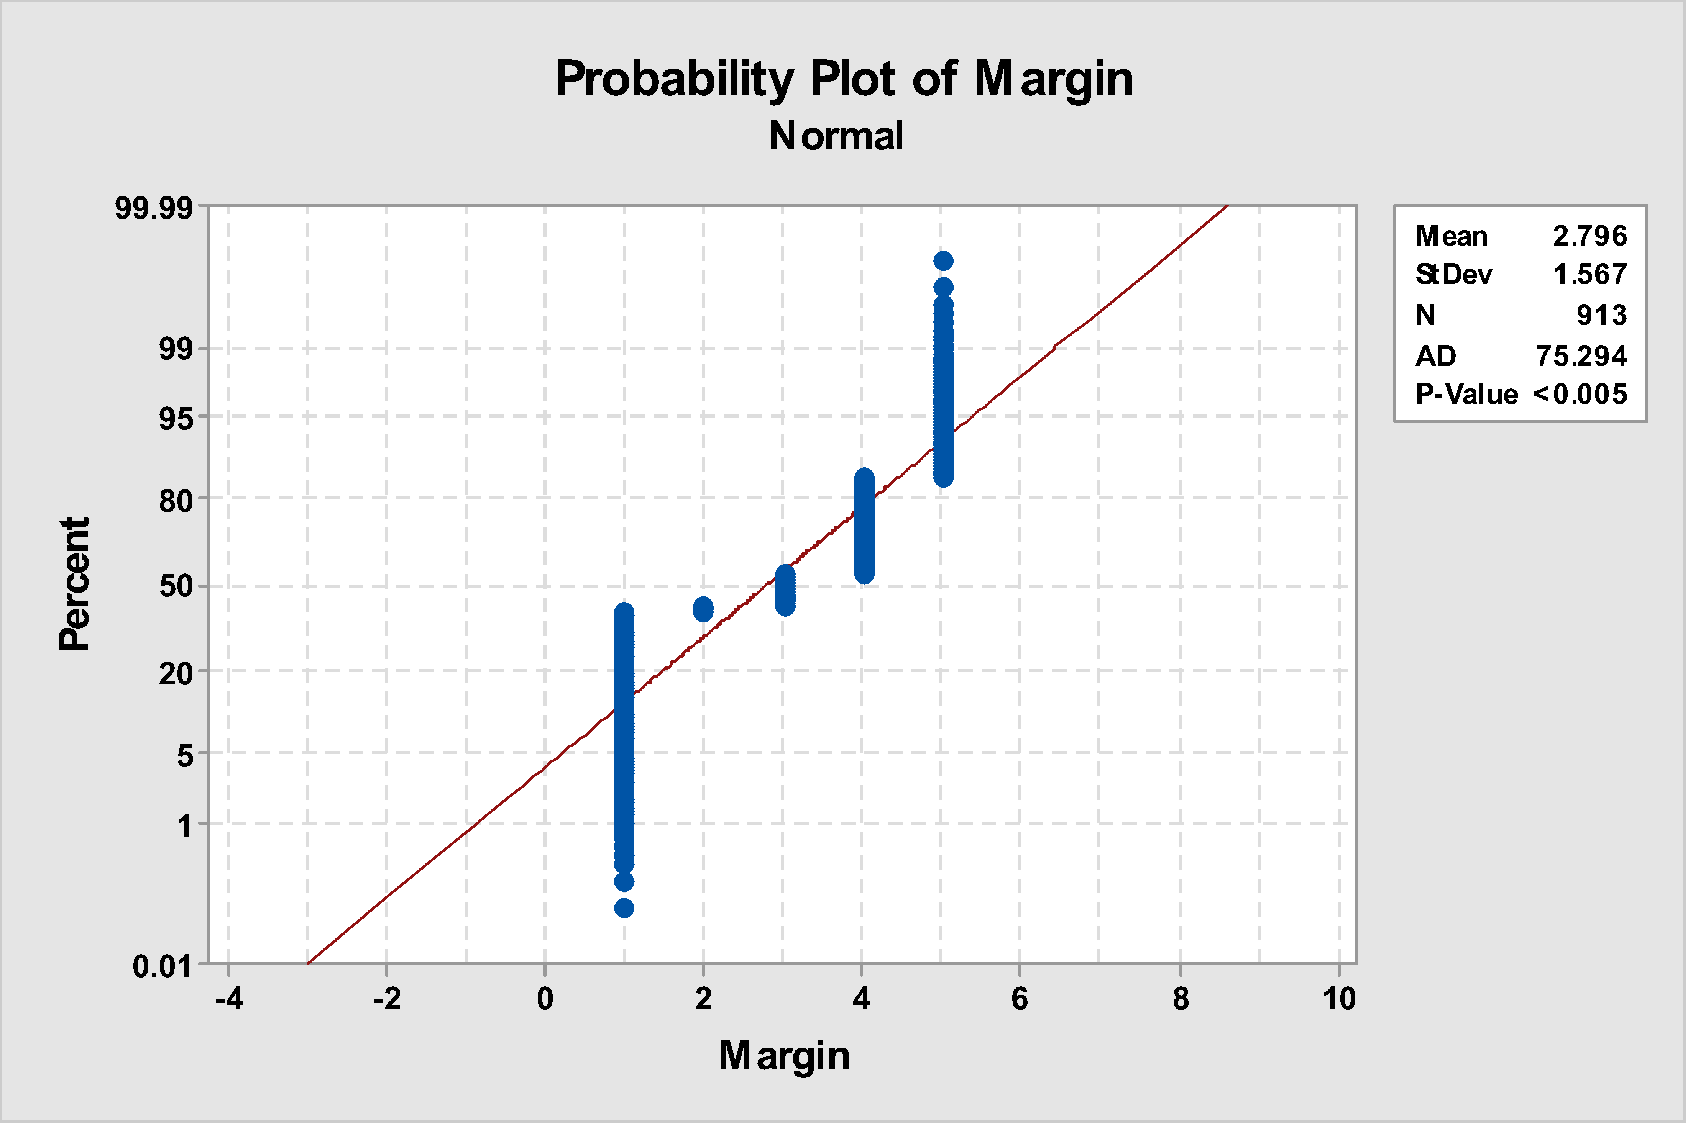
\includegraphics[width=\textwidth]{margin-probability}
            \caption{Margin probability}
            \label{fig:margin-probability}
          \end{minipage}
        \end{figure}

      \subsubsection{Outliers}
        There does not appear to be any outliers within this attribute however it does contain 48 missing values. Due to it again being a nominal value the central tendancy for these values should be the mode.

      \subsubsection{Predictive}
        Once again, it can be observed in figure \ref{fig:margin-severity-correlation} that a higher score of margin will correlate with a higher chance of a malignant severity.

        \begin{figure}[H]
          \centering
          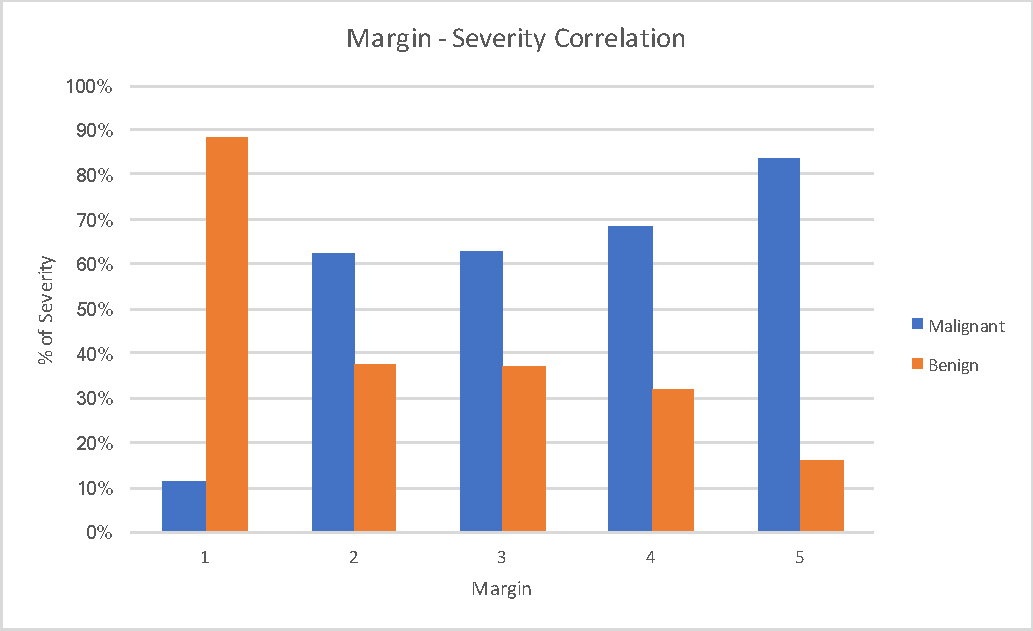
\includegraphics[width=0.6\textwidth]{margin-severity-correlation}
          \caption{Margin - Severity correlation}
          \label{fig:margin-severity-correlation}
        \end{figure}

    \subsection{Density}
      \subsubsection{Measurement}
        This attribute is used to describe the density of the mass on an ordinal scale. A lower score indicates a higher density, which has been shown to be a significant predictor of breast cancer \citep{woods2011mammographic}. Below are the descriptors used to score masses onto the ordinal scale.

        \begin{enumerate}[label=\arabic*)]
          \item High
          \item ISO (Isodense)
          \item Low
          \item Fat-containing
        \end{enumerate}

      \subsubsection{Distribution}
        As shown in figure \ref{fig:margin-histogram}, the distribution of values in the density attribute appear to be non-normal and skewed to the right.

        \begin{figure}[H]
          \centering
          \begin{minipage}[b]{0.45\textwidth}
            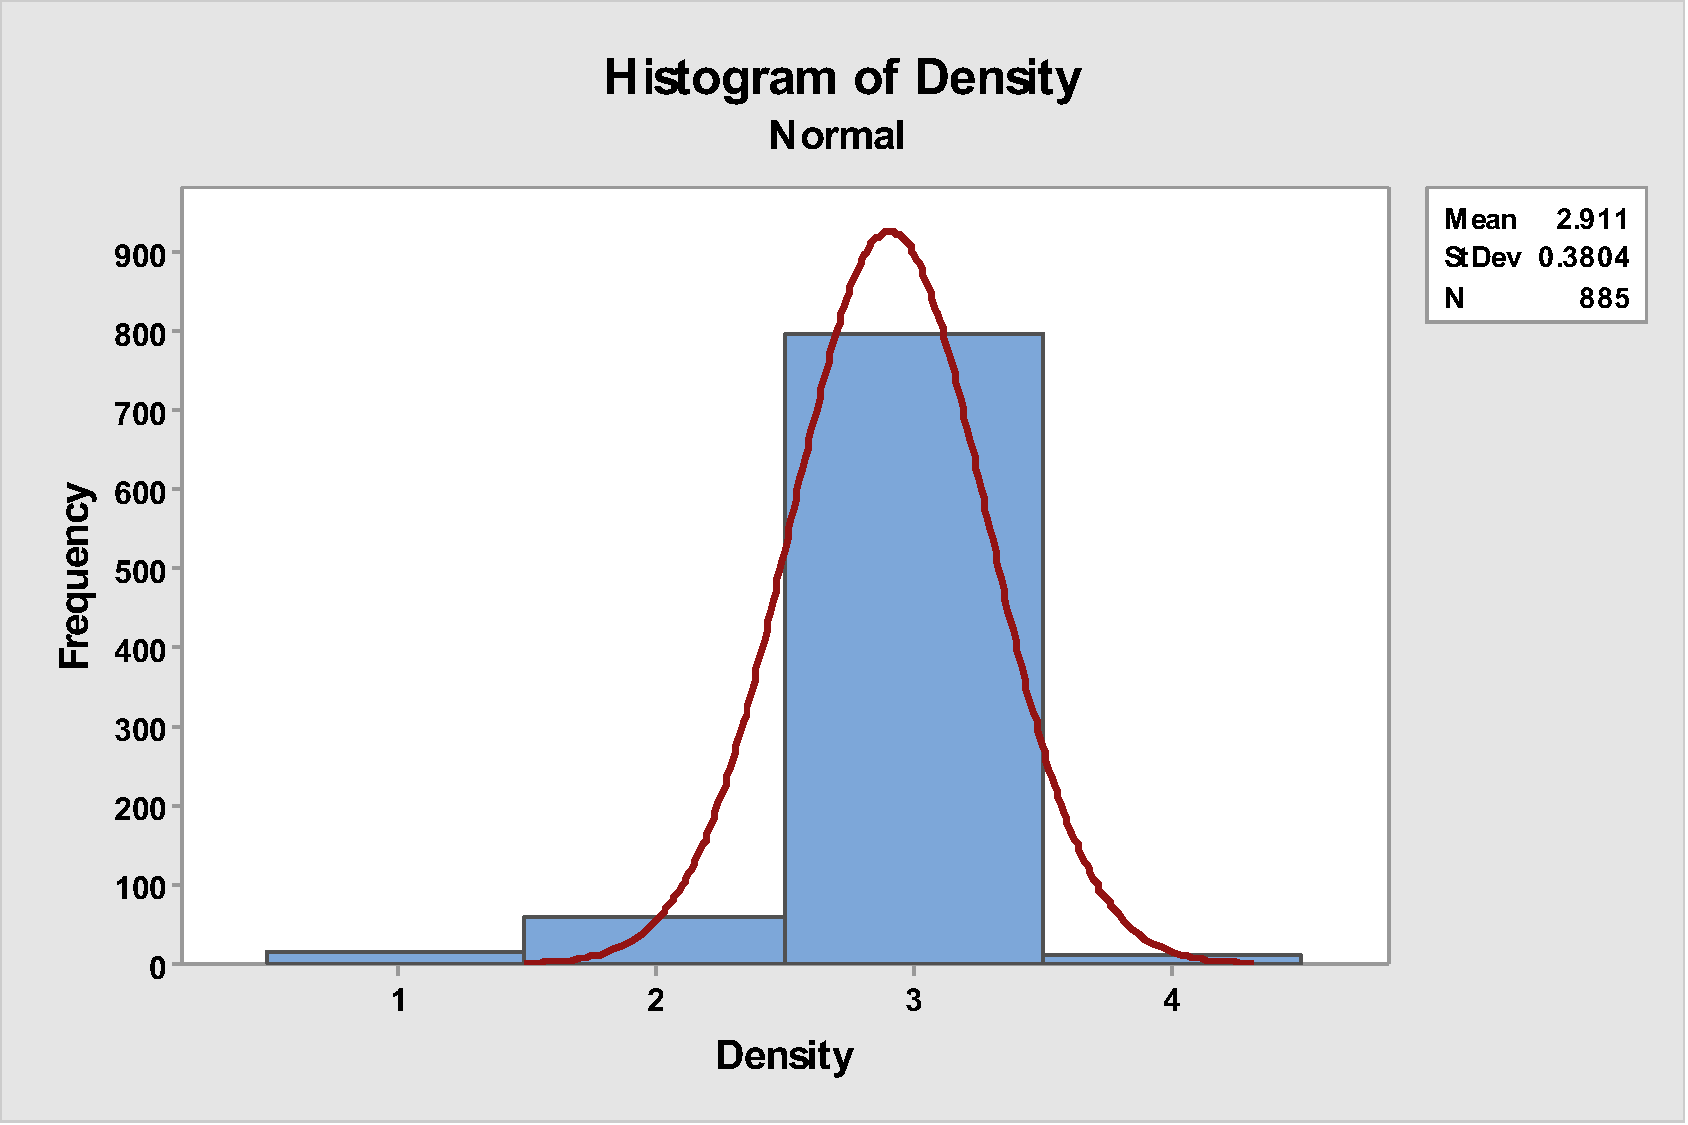
\includegraphics[width=\textwidth]{density-histogram}
            \caption{Density histogram}
            \label{fig:density-histogram}
          \end{minipage}
          \hfill
          \begin{minipage}[b]{0.45\textwidth}
            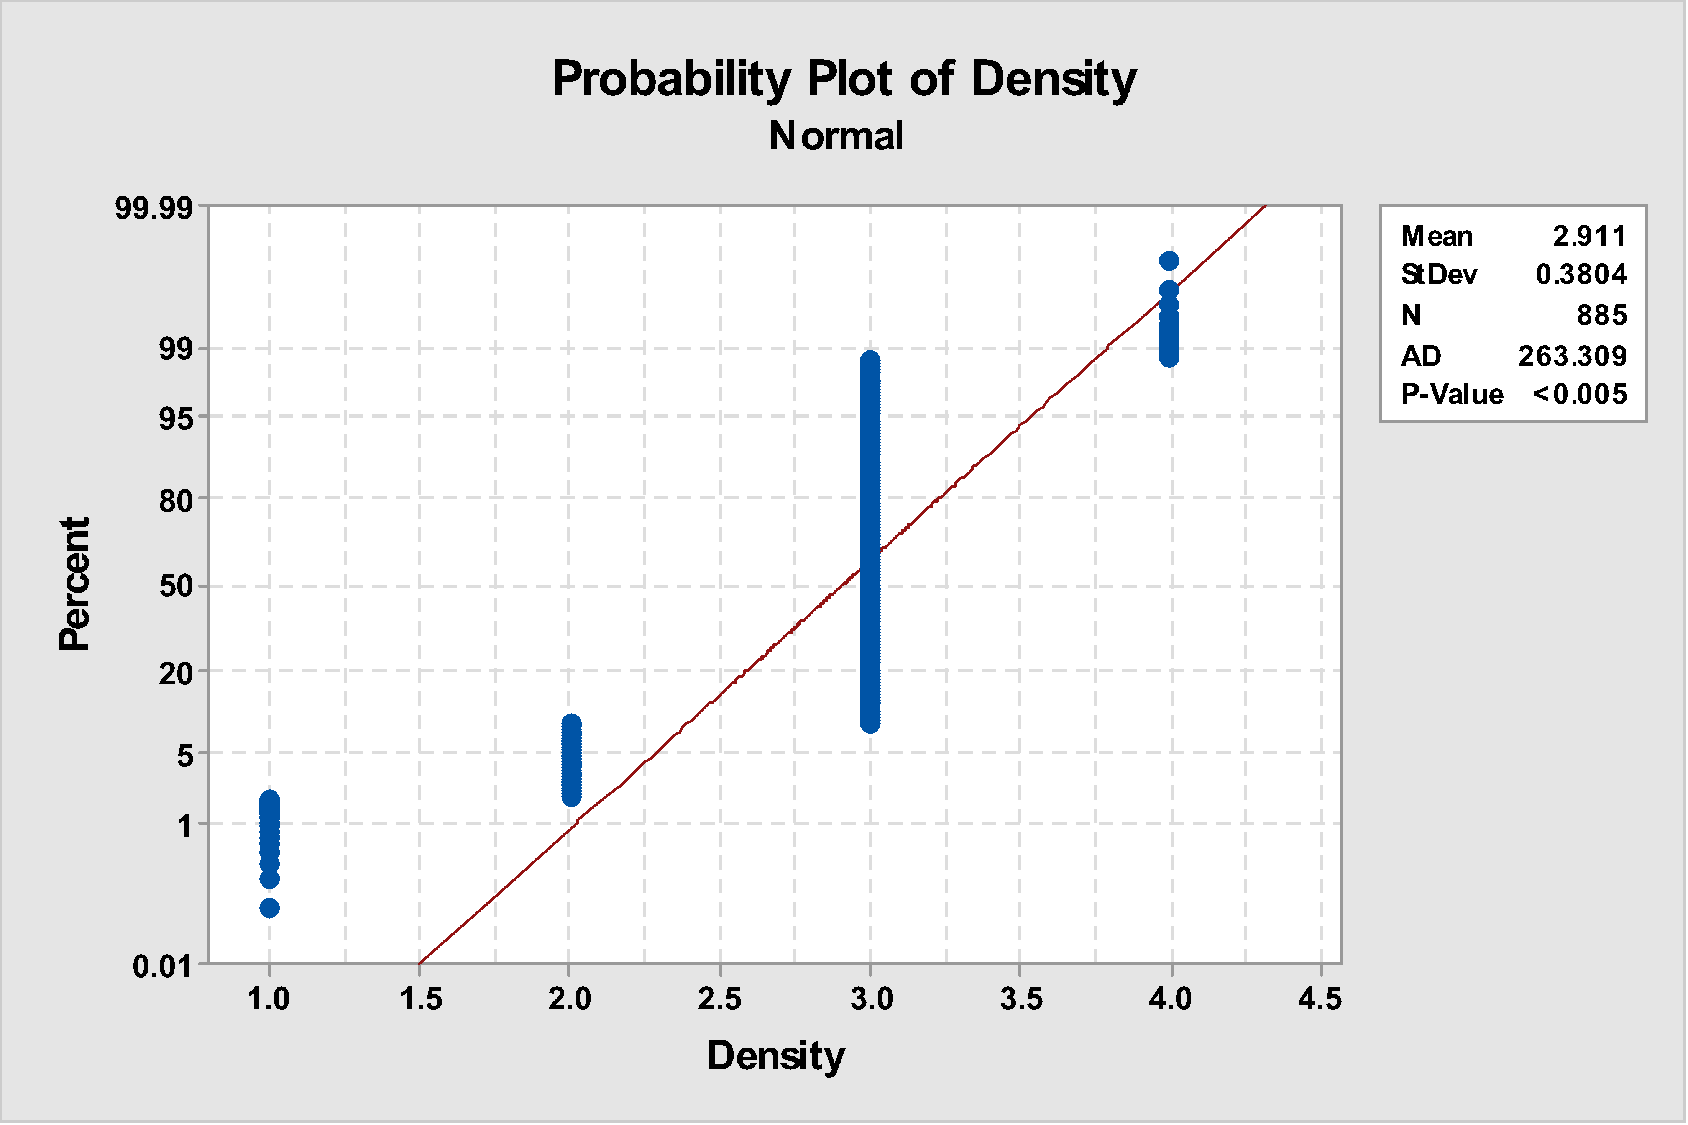
\includegraphics[width=\textwidth]{density-probability}
            \caption{Density probability}
            \label{fig:density-probability}
          \end{minipage}
        \end{figure}

      \subsubsection{Outliers}
        While there is no outliers within this attribute, there are 76 missing values. The central tendancy for replacing these values should be the median due to the data type being ordinal.

      \subsubsection{Predictive}
        Figure \ref{fig:density-severity-correlation} below shows that in contrary to \cite{woods2011mammographic}, the dataset provided does not seem to have a significant correlation between high-density masses and a malignant severity.

        \begin{figure}[H]
          \centering
          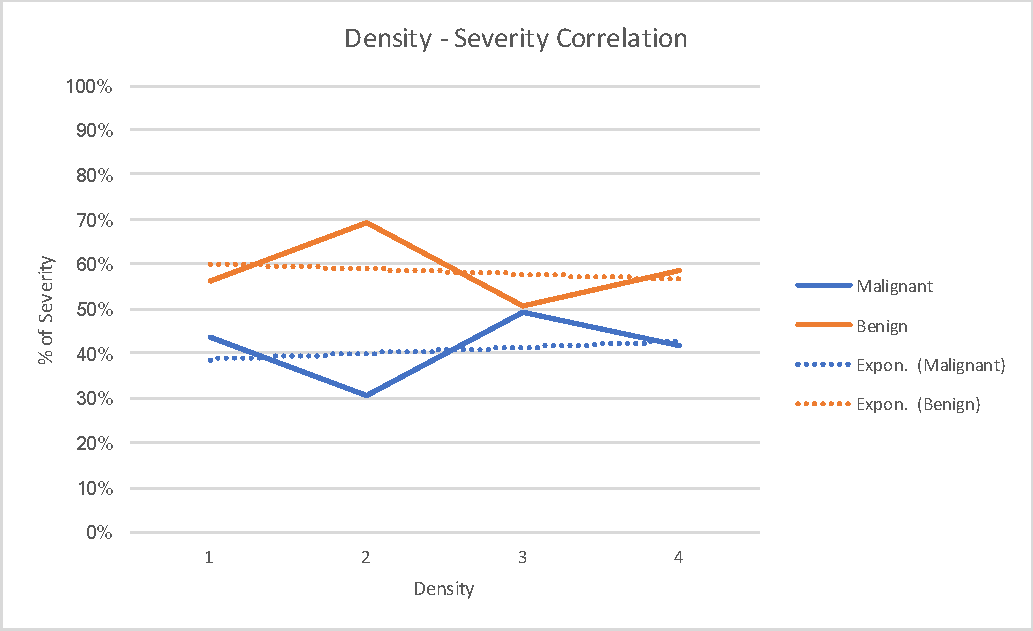
\includegraphics[width=0.6\textwidth]{density-severity-correlation}
          \caption{Density - Severity correlation}
          \label{fig:density-severity-correlation}
        \end{figure}

    \subsection{Severity}
      This field is known as a goal field and is a binomial type. This field contains the classification of the instances. In order to make the dataset more compatible with WEKA processing, the original values of ‘0’ and ‘1’ have been replaced by ‘$-$’ and ‘+’ respectively.

\section{Classifier Evaluation}
  In this section the two different classifier types will be evaluated for their suitability in the task of classifying the mammographic dataset.

  \subsection{Decision Tree}
    \subsubsection{Strengths}
      \paragraph{Speed.}
        Decision trees are often a lot faster than neural networks (once trained), this is due to the fact that the algorithm creates a set of simple rules which are very quick to execute, and can be implemented in any programming language.
      \paragraph{Interpretability.}
        Again due to the nature of decision trees, the resulting classifier is very easy to interpret due to the creation of simple rules. It then provides insights on the relationships between the attributes and the classes.
      \paragraph{Feature selection.}
        Decision trees are good with noisy data due to the fact that they are able to completely ignore certain attributes if they are not deemed important enough as a contributor to classification.

    \subsubsection{Weaknesses}
      \paragraph{Nonlinear interactions.}
        Decision trees are not as good at handling data with nonlinear relationships due to their structure. If the relationship between two attributes is not definable in a simple rule then a decision tree will not be able to

  \subsection{Artificial Neural Network}
    \subsubsection{Strengths}
      \paragraph{Nonlinear interactions.}
        ANNs are very good at handling abstract relationships in datasets, therefore if there is any information contained in the data which can be inferred, then it is likely that a neural network could make use of this inferrance.

    \subsubsection{Weaknesses}
      \paragraph{No feature Selection.}
        ANNs automatically use every piece of input data given to them. If one or more of the attributes contain noisy data or do not provide much value, then these could hinder the performance of the classifier unless they are removed manually as a pre-processing step.

      \paragraph{Black box.}
        ANNs do not provide a systematical view of how a classification is made (it can be done given the proper functions and weight/bias values, however calculating it manually could take a very long time). This is not useful when trying to determine the relationships between different attributes in the data.

      \paragraph{Speed.}
        The time taken for both training and classification are often higher in neural netwoks especially when the complexity of the network structure is increased (i.e. by adding more neurons and/or hidden layers).

  \subsection{Prediction}
    In order to predict the outcome of which classifier is most suited for this task, it must be made clear how the dataset will interact with the classifier.
    In section \ref{data-set-analysis} it was shown that the dataset has some clear links between attributes and classifications (such as a high correlation between age and severity shown in figure \ref{fig:age-severity-correlation}). Due to the nature of decision trees which are more able to deal with data that have a clear link between attributes and classification, it could be presumed that the decision tree classifier would be more suited for this task than an artificial neural network.

\section{Initial Experiments - Pre-processing}
  In this section the pre-processing steps for the dataset will be explained and a series of initial experiments prior to pre-processing will be carried out to find the best strategy for classifying data.

  \subsection{Missing values}
    As explained in section \ref{data-set-analysis}, each parameter has its own central tendancy due to their different distributions and data types. The strategy for missing values will be to replace them with the central tendancy for each parameter. As there is only 961 instances within the dataset it would not be benefitial to remove any instances with missing values as the other parameters would then suffer from real data being removed from them.

  \subsection{Outliers}
    As previously explored in section \ref{birad-outlier}, the main outlier is within the BI-RADS attribute and has been replaced with the central tendancy. Once again if this instance were to be removed (when it is only likely there due to human input error) then the dataset could risk losing valuable data for other parameters in that instance.

  \subsection{Results}
    Below are the results from some initial experiments done prior to pre-processing of data (aside from removing the outlier mentioned in section \ref{birad-outlier}).

    \subsubsection{Decision Tree}
      \begin{table}[H]
        \begin{subtable}{0.5\linewidth}
          \centering
          \caption{}
            \begin{tabular}{c|c}
            \toprule
            \multicolumn{1}{l|}{Confidence} & \multicolumn{1}{l}{Accuracy (\%)} \\
            \midrule
            0.05  & 82.2 \\
            0.1   & 82.16 \\
            0.15  & 82.19 \\
            0.2   & 82.27 \\
            0.25  & 82.19 \\
            0.3   & \textbf{82.33} \\
            0.35  & 82.31 \\
            0.4   & 82.12 \\
            \bottomrule
            \end{tabular}%
        \end{subtable}
        \begin{subtable}{0.5\linewidth}
          \centering
          \caption{}
            \begin{tabular}{c|c}
            \toprule
            Confidence & Accuracy (\%)\\
            \midrule
            0.29  & 82.29 \\
            0.295 & 82.31 \\
            0.299 & 82.33 \\
            0.305 & \textbf{82.33} \\
            0.31  & \textbf{82.33} \\
            0.32  & \textbf{82.33} \\
            0.34  & 82.31 \\
            0.36  & 82.32 \\
            0.38  & 82.28 \\
            \bottomrule
            \end{tabular}%
          \label{tab:dt-2}%
        \end{subtable}
        \caption{Tuning confidence}
        \label{tab:dt-1}%
      \end{table}%

      \begin{table}[H]
        \begin{subtable}{0.5\linewidth}
          \centering
          \caption{}
            \begin{tabular}{c|c}
            \toprule
            \multicolumn{1}{l|}{Min Objects} & \multicolumn{1}{l}{Accuracy (\%)} \\
            \midrule
            2     & 82.33 \\
            5     & 82.30 \\
            10    & 82.24 \\
            15    & 82.54 \\
            18    & 82.83 \\
            19    & 82.99 \\
            20    & 83.00 \\
            21    & 83.04 \\
            22    & 82.98 \\
            30    & 83.16 \\
            35    & 83.53 \\
            40    & 83.73 \\
            45    & 83.80 \\
            50    & \textbf{83.82} \\
            60    & 83.04 \\
            70    & 82.82 \\
            \bottomrule
            \end{tabular}%
        \end{subtable}
        \begin{subtable}{0.5\linewidth}
          \centering
          \caption{}
            \begin{tabular}{c|c}
            \toprule
            MinNumObj & Accuracy (\%) \\
            \midrule
            45    & 83.80 \\
            46    & \textbf{83.84} \\
            47    & \textbf{83.84} \\
            48    & 83.81 \\
            49    & 83.81 \\
            50    & 83.82 \\
            51    & 83.79 \\
            52    & 83.79 \\
            53    & 83.70 \\
            54    & 83.62 \\
            55    & 83.62 \\
            \bottomrule
            \end{tabular}%
        \end{subtable}
        \label{tab:mno-1}%
        \caption{Minimum number of objects tuning (C=0.3)}
      \end{table}%

      \begin{table}[H]
        \begin{subtable}{0.5\linewidth}
          \centering
          \caption{}
          \begin{tabular}{c|c}
            \toprule
            MinNumObj & Accuracy (\%) \\
            \midrule
            46    & \textbf{83.84} \\
            \midrule
            100   & 82.50 \\
            110   & 82.50 \\
            120   & 82.23 \\
            130   & 81.89 * \\
            140   & 81.89 * \\
            150   & 81.89 * \\
            160   & 81.89 * \\
            170   & 81.89 * \\
            180   & 81.89 * \\
            190   & 81.89 * \\
            200   & 81.89 * \\
            \bottomrule
          \end{tabular}%
        \end{subtable}
        \begin{subtable}{0.5\linewidth}
          \centering
          \caption{}
            \begin{tabular}{c|c}
            \toprule
            MinNumObj & Accuracy (\%) \\
            \midrule
            46    & \textbf{83.84} \\
            \midrule
            120   & 82.23 \\
            121   & 82.03 * \\
            122   & 82.05 * \\
            123   & 82.03 * \\
            124   & 81.99 * \\
            125   & 81.92 * \\
            126   & 81.88 * \\
            127   & 81.89 * \\
            128   & 81.89 * \\
            129   & 81.89 * \\
            130   & 81.89 * \\
            \bottomrule
            \end{tabular}%
        \end{subtable}
        \caption{Finding most pruned tree}
        \label{tab:dt-mpt}%
      \end{table}%

    \subsubsection{Artificial Neural Network}
      \begin{table}[H]
        \centering
        \caption{Learning rate accuracy from 200-3000 epochs}
          \begin{tabular}{r|rrrrr}
          \toprule
          \multicolumn{1}{r}{} & \multicolumn{5}{|c}{Learning Rate} \\
          & 0.1   & 0.3   & 0.5   & 0.7   & 0.9 \\
          \midrule
              Epochs & \multicolumn{5}{|c}{Accuracy (\%)} \\
          \midrule
          200   & \textbf{81.19} & 80.72 & 80.49 & 80.21 & 79.93 \\
          250   & 80.19 & \textbf{80.99} & 80.58 & 80.39 & 79.97 \\
          350   & 81.27 & \textbf{81.36} & 81.01 & 80.5  & 80.2 \\
          450   & 81.49 & \textbf{81.52} & 80.87 & 80.55 & 80.39 \\
          550   & \textbf{81.72} & 81.56 & 81.13 & 81.08 & 80.74 \\
          650   & \textbf{82.05} & 81.7  & 81.34 & 81.27 & 80.92 \\
          750   & \textbf{82.04} & 81.68 & 81.59 & 81.37 & 81.14 \\
          850   & \textbf{82.16} & 81.77 & 81.76 & 81.52 & 81.16 \\
          950   & \textbf{82.12} & 81.9  & 81.71 & 81.66 & 81.32 \\
          1050  & \textbf{82.13} & 81.96 & 81.84 & 81.77 & 81.28 \\
          1150  & 81.99 & \textbf{82} & 81.8  & 81.81 & 81.34 \\
          1500  & 82.08 & \textbf{82.22} & 81.84 & 81.92 & 81.5 \\
          2000  & 82.23 & \textbf{82.32} & 81.88 & 81.94 & 81.74 \\
          3000  & \textbf{82.25} & 82.24 & 81.84 & 81.86 & 81.69 \\
          \bottomrule
          \end{tabular}%
        \label{tab:addlabel}%
      \end{table}%

      \begin{table}[H]
        \centering
        \caption{Momentum accuracy from 200-3000 epochs (LR=0.4, HL=A)}
          \begin{tabular}{r|rrrrr}
          \toprule
                & \multicolumn{5}{c}{Momentum} \\
          \midrule
          \multicolumn{1}{l|}{Epochs} & 0.1   & 0.3   & 0.5   & 0.7   & 0.9 \\
          \midrule
          200   & 80.59 & \textbf{80.66} & 80.24 & 79.92 & 79.31 \\
          300   & \textbf{81.07} & 80.96 & 80.55 & 80.46 & 79.34 \\
          400   & \textbf{81.31} & 81.17 & 80.68 & 80.55 & 79.49 \\
          500   & 81.33 & \textbf{81.36} & 80.96 & 80.72 & 79.39 \\
          600   & 81.45 & \textbf{81.51} & 81.22 & 80.98 & 79.5 \\
          700   & 81.55 & \textbf{81.64} & 81.38 & 81.15 & 79.48 \\
          800   & 81.52 & \textbf{81.71} & 81.52 & 81.41 & 79.52 \\
          900   & 81.69 & \textbf{81.72} & 81.53 & 81.46 & 79.38 \\
          1000  & \textbf{81.85} & 81.78 & 81.55 & 81.42 & 79.46 \\
          1100  & 81.89 & \textbf{81.98} & 81.61 & 81.63 & 79.66 \\
          1500  & \textbf{82.07} & 82.04 & 81.69 & 81.61 & 79.9 \\
          2000  & \textbf{82.06} & 82.03 & 81.78 & 81.66 & 80.05 \\
          3000  & 81.98 & \textbf{82.05} & 81.81 & 81.64 & 80 \\
          \bottomrule
          \end{tabular}%
        \label{tab:addlabel}%
      \end{table}%

      \begin{table}[H]
        \centering
        \caption{Two hidden layer ANN structure (LR=0.4, M=0.2, E=950)}
          \begin{tabular}{c|rrrrr}
            \toprule
              & \multicolumn{5}{c}{Second Layer Neurons} \\
            \midrule
              \multicolumn{1}{c|}{First Layer Neurons} & 1     & 2     & 3     & 4     & 5 \\
            \midrule
              1 & 82.34 & 82.25 & 82.43 & 82.64 & \textbf{82.67} \\
              2 & 81.78 & 81.89 & 82.29 & 82.06 & \textbf{82.38} \\
              3 & 81.02 & 81.32 & 81.79 & 81.96 & \textbf{82.01} \\
              4 & 80.66 & 81.38 & 80.92 & 80.99 & \textbf{81.07} \\
              5 & 80.55 & 80.53 & \textbf{81.29} & 81.02 & 80.7 \\
            \bottomrule
          \end{tabular}%
        \label{tab:addlabel}%
      \end{table}%

      \begin{table}[H]
        \centering
        \caption{Learning rate impact on accuracy from 250-3000 epochs (M=0.2, HL=1)}
          \begin{tabular}{r|rrrrr}
          \toprule
                & \multicolumn{5}{c}{Learning Rate} \\
          \midrule
          \multicolumn{1}{l|}{Epochs} & 0.1   & 0.3   & 0.5   & 0.7   & 0.9 \\
          \midrule
          250   & 81.73 & \textbf{81.88} & 81.85 & 81.87 & 81.8 \\
          350   & \textbf{82.27} & 82.24 & 82.21 & 82.19 & 82.23 \\
          450   & \textbf{82.58} & 82.49 & 82.39 & 82.33 & 82.35 \\
          550   & 82.55 & \textbf{82.61} & 82.58 & 82.41 & 82.33 \\
          650   & \textbf{82.73} & 82.7  & 82.72 & 82.66 & 82.45 \\
          750   & 82.77 & 82.8  & \textbf{82.83} & 82.74 & 82.5 \\
          850   & 82.79 & \textbf{82.93} & 82.88 & 82.66 & 82.5 \\
          950   & 82.89 & \textbf{83} & 82.87 & 82.78 & 82.55 \\
          1050  & 82.9  & \textbf{83} & 82.89 & 82.83 & 82.61 \\
          1150  & 82.89 & \textbf{83} & 82.87 & 82.88 & 82.69 \\
          1500  & 82.98 & 82.99 & \textbf{83.09} & 83    & 82.87 \\
          2000  & 83.08 & 83.15 & \textbf{83.19} & 83.14 & 83 \\
          3000  & \textbf{83.25} & 83.19 & 83.21 & 83.18 & 83.01 \\
          \bottomrule
          \end{tabular}%
        \label{tab:addlabel}%
      \end{table}%

\newpage
\section{Main Experiments}
  In this section the experiments will be carried out which indicate the best possible classifier for both Decision trees and Artificial Neural Networks. These results will include pre-processing steps including replacing missing values with the central tendancy and replacing nominal values with their text values to ensure they are processed correctly. Throughout all experiments a 10-fold cross-validation train/test set will be used, this will make use of every instance of the data in training and testing which is vital due to the low number of instances in the dataset.

  \subsection{Decision tree}
    As a result of the information presented in section \ref{res-destrees}, a series of experiments will be carried out to find the optimal parameters for training when a J48 decision tree algorithm is used on the mamographical dataset. In this section two trees will be laid out, the first being the tree with the highest classification accuracy and the second being the one which is most pruned but not significantly worse than the highest accuracy tree.

    \subsubsection{Plan}
      The first series of experiments will be to find the optimal confidence setting, by iterating through different values at gradually smaller intervals. Once the optimal confidence value is found, then the Minimum number of Object parameter will also need to be tuned in order to find its optimal value. Once again this can be done by increasing the value at set increments and reducing the size of the increments around values which show the highest accuracy results.

    \subsubsection{Execution} \label{dt-execution}
      Tables \ref{tab:dt-con-a}, \ref{tab:dt-con-b} \& \ref{tab:dt-con-c} illustrate the process of finding the optimal confidence parameter value. As seen in table \ref{tab:dt-con-c} the optimal confidence value (with the minimum number of objects parameter set to its default of 2) is 0.247, which gives an accuracy score of 82.99\%. As many of the accuracy values are repeating with the 3 decimal point intervals seen in table \ref{tab:dt-con-c}, there is no reason to search through smaller intervals.

      \begin{table}[H]
          \caption{Confidence tuning}
          \begin{subtable}{.34\linewidth}
            \centering
            \caption{}
            \begin{tabular}{c|c}
              \toprule
              \multicolumn{1}{c|}{Confidence} & \multicolumn{1}{c}{Accuracy (\%)} \\
              \midrule
              0.05  & 82.26 \\
              0.10  & 82.81 \\
              0.15  & 82.79 \\
              0.20  & 82.80 \\
              0.25  & \textbf{82.99} \\
              0.30  & 82.92 \\
              0.35  & 82.57 \\
              0.40  & 82.42 \\
              0.45  & 82.30 \\
              0.50  & 82.19 \\
              0.55  & 82.14 \\
              0.60  & 82.14 \\
              0.65  & 82.14 \\
              0.70  & 82.14 \\
              0.75  & 82.14 \\
              0.80  & 82.14 \\
              0.85  & 82.14 \\
              0.90  & 82.14 \\
              0.95  & 82.14 \\
              1.00  & 82.14 \\
              \bottomrule
            \end{tabular}
            \label{tab:dt-con-a}
          \end{subtable}%
          \begin{subtable}{.34\linewidth}
            \centering
            \caption{}
            \begin{tabular}{c|c}
              \toprule
              \multicolumn{1}{c|}{Confidence} & \multicolumn{1}{c}{Accuracy (\%)} \\
              \midrule
              0.21  & 82.88 \\
              0.22  & 82.88 \\
              0.23  & 82.93 \\
              0.24  & 82.97 \\
              0.25  & \textbf{82.99} \\
              0.26  & 82.93 \\
              0.27  & 82.93 \\
              0.28  & 82.93 \\
              0.29  & 82.89 \\
              0.30  & 82.92 \\
              0.31  & 82.85 \\
              0.32  & 82.85 \\
              0.33  & 82.81 \\
              0.34  & 82.64 \\
              0.35  & 82.57 \\
              \bottomrule
            \end{tabular}
            \label{tab:dt-con-b}
          \end{subtable}%
          \begin{subtable}{.34\linewidth}
            \centering
            \caption{}
            \begin{tabular}{c|c}
              \toprule
              \multicolumn{1}{l|}{Confidence} & \multicolumn{1}{l}{Accuracy (\%)} \\
              \midrule
              0.245 & 82.97 \\
              0.246 & 82.98 \\
              0.247 & \textbf{82.99} \\
              0.248 & \textbf{82.99} \\
              0.249 & \textbf{82.99} \\
              0.250 & \textbf{82.99} \\
              0.251 & 82.96 \\
              0.252 & 82.93 \\
              0.253 & 82.93 \\
              0.254 & 82.93 \\
              0.255 & 82.93 \\
              \bottomrule
            \end{tabular}
          \label{tab:dt-con-c}
          \end{subtable}%
        \label{tab:dt-con}
      \end{table}

      Tables \ref{tab:dt-minobj-a} and \ref{tab:dt-minobj-b} show the process of finding the optimal parameter value for the minimum number of objects, with the confidence value set to the optimal 0.247. Specifically table \ref{tab:dt-minobj-b} shows that the optimal value is 52 with an accuracy score of 83.95\%. As this parameter is an integer scale there is no way to process smaller intervals.

      \begin{table}[H]
        \caption{Minumum Number of Objects tuning}
        \begin{subtable}{.5\linewidth}
          \centering
          \caption{}
          \begin{tabular}{c|c}
          \toprule
          \multicolumn{1}{l|}{Min Objects} & \multicolumn{1}{l}{Accuracy (\%)} \\
          \midrule
          2     & 82.99 \\
          5     & 82.99 \\
          10    & 83.05 \\
          15    & 83.56 \\
          20    & 83.67 \\
          25    & 83.71 \\
          30    & 83.60 \\
          35    & 83.75 \\
          40    & 83.75 \\
          45    & 83.83 \\
          50    & \textbf{83.90} \\
          55    & 83.07 \\
          60    & 81.79 \\
          65    & 81.79 \\
          70    & 81.78 \\
          75    & 81.83 \\
          80    & 81.83 \\
          85    & 81.83 \\
          90    & 81.83 \\
          95    & 81.83 \\
          100   & 81.83 \\
          \bottomrule
          \end{tabular}
          \label{tab:dt-minobj-a}
        \end{subtable}
        \begin{subtable}{.5\linewidth}
          \centering
          \caption{}
          \begin{tabular}{c|c}
            \toprule
            \multicolumn{1}{l|}{Min Objects} & \multicolumn{1}{l}{Accuracy (\%)} \\
            \midrule
            45    & 83.83 \\
            46    & 83.80 \\
            47    & 83.86 \\
            48    & 83.91 \\
            49    & 83.90 \\
            50    & 83.90 \\
            51    & 83.94 \\
            52    & \textbf{83.95} \\
            53    & 83.85 \\
            54    & 83.66 \\
            55    & 83.07 \\
            \bottomrule
            \end{tabular}
          \label{tab:dt-minobj-b}
        \end{subtable}
        \label{tab:dt-minobj}
      \end{table}

      Tables \ref{tab:dt-minobj-prun-a} and \ref{tab:dt-minobj-prun-b} show the process of finding the most pruned tree which is not significantly worse than the tree with the highest classification accuracy which was found in the previous paragraph. Specifically table \ref{tab:dt-minobj-prun-b} shows that the most pruned tree which is not significantly worse is one with 56 minumum number of objects. Again this parameter is an integer scale so there is no way to find smaller intervals.

      \begin{table}[H]
        \caption{Finding the most pruned tree}
        \begin{subtable}{.5\linewidth}
          \centering
          \caption{}
          \begin{tabular}{c|c}
            \toprule
            \multicolumn{1}{l|}{Min Objects} & \multicolumn{1}{l}{Accuracy (\%)} \\
            \midrule
            52    & \textbf{83.95} \\
            \midrule
            50    & 83.90 \\
            60    & 81.79 * \\
            70    & 81.78 * \\
            80    & 81.83 * \\
            90    & 81.83 * \\
            100   & 81.83 * \\
            110   & 81.77 * \\
            120   & 81.47 * \\
            130   & 81.49 * \\
            140   & 81.49 * \\
            150   & 81.49 * \\
            \bottomrule
          \end{tabular}
        \label{tab:dt-minobj-prun-a}
        \end{subtable}
        \begin{subtable}{.5\linewidth}
          \centering
          \caption{}
          \begin{tabular}{c|c}
            \toprule
            \multicolumn{1}{l|}{Min Objects} & \multicolumn{1}{l}{Accuracy (\%)} \\
            \midrule
            52    & \textbf{83.95} \\
            \midrule
            50    & 83.90 \\
            51    & 83.94 \\
            53    & 83.85 \\
            54    & 83.66 \\
            55    & 83.07 \\
            56    & 82.47 \\
            57    & 82.08 * \\
            58    & 81.83 * \\
            59    & 81.83 * \\
            60    & 81.79 * \\
            \bottomrule
          \end{tabular}
          \label{tab:dt-minobj-prun-b}
        \end{subtable}
        \label{tab:dt-minobj-prun}
      \end{table}

  \subsection{Artificial Neural Network}
    As a result of the information presented in section \ref{ann}, a series of experiments will be carried out to find the optimal parameters for training when an Artificial neural network is used on the mamographical dataset. In this section two network structures will be laid out, the first being the one with a single hidden layer of neurons and the second being one with two hidden layers of neurons.

    \subsubsection{Plan}
      In order to find the best structure for an ANN with both 1 and 2 hidden layers of neurons, first the optimal learning parameters must be found. To do this a series of experiments must be run with different learning rate and momentum values, each over a long series of training times. At first intervals of 0.2 will be used between learning rate / momentum values as the more optimal value can be determined once the best training time is found.

      Once the optimal training parameters are found another series of experiments with different combinations of ANN structures will be carried out, which make use of the training parameters found in the previous experiments.

    \subsubsection{Execution} \label{ann-ex}
      Table \ref{tab:ann-lr-a} shows that the best learning rate over the majority of training times is 0.1, and that a training time of 700 epochs is the most optimal time with an accuracy of 82.63\%. Using this as a basis, table \ref{tab:ann-lr-b} shows a wider scope of learning rates where it can be observed that 0.1 is still the most optimal value. Table \ref{tab:ann-lr-c} shows finer intervals around the 0.1 value and again highlights that it is still the best value. Finally, table \ref{tab:ann-lr-d} shows the two neighbor values which still give lower scores than the 0.1 value. Therefore it is proven that 0.1 is the optimal learning rate value.

      \singlespacing
      \begin{table}[H]
        \centering
        \caption{Learning rate tuning}
        \begin{subtable}{.49\linewidth}
          \centering
          \caption{}
          \begin{tabular}{c|ccccc}
            \toprule
                  & \multicolumn{5}{c}{Learning Rate} \\
            \midrule
                  & \multicolumn{1}{c|}{0.1} & \multicolumn{1}{c|}{0.3} & \multicolumn{1}{c|}{0.5} & \multicolumn{1}{c|}{0.7} & 0.9 \\
            \midrule
            Epochs & \multicolumn{5}{c}{Accuracy (\%)} \\
            \midrule
            100   & \textbf{82.3} & 82.29 & 82.13 & 81.84 & 81.79 \\
            200   & 82.31 & \textbf{82.33} & 82.17 & 81.87 & 81.85 \\
            300   & \textbf{82.47} & 82.39 & 82.04 & 81.9  & 81.63 \\
            400   & \textbf{82.53} & 82.37 & 81.93 & 81.8  & 81.54 \\
            500   & \textbf{82.54} & 82.36 & 81.88 & 81.75 & 81.56 \\
            600   & \textbf{82.6} & 82.27 & 81.86 & 81.72 & 81.54 \\
            700   & \textbf{82.63} & 82.21 & 81.83 & 81.68 & 81.58 \\
            800   & \textbf{82.62} & 82.18 & 81.83 & 81.61 & 81.5 \\
            900   & \textbf{82.62} & 82.15 & 81.8  & 81.62 & 81.45 \\
            1000  & \textbf{82.6} & 82.12 & 81.79 & 81.6  & 81.37 \\
            1100  & \textbf{82.54} & 82.1  & 81.78 & 81.59 & 81.36 \\
            1200  & \textbf{82.55} & 82.08 & 81.77 & 81.56 & 81.31 \\
            1300  & \textbf{82.53} & 82.06 & 81.73 & 81.52 & 81.28 \\
            1400  & \textbf{82.53} & 82.01 & 81.72 & 81.5  & 81.27 \\
            1500  & \textbf{82.52} & 82.01 & 81.73 & 81.46 & 81.25 \\
            1600  & \textbf{82.53} & 81.96 & 81.71 & 81.43 & 81.23 \\
            1700  & \textbf{82.51} & 81.89 & 81.73 & 81.4  & 81.24 \\
            1800  & \textbf{82.51} & 81.92 & 81.73 & 81.44 & 81.26 \\
            1900  & \textbf{82.51} & 81.9  & 81.76 & 81.44 & 81.27 \\
            2000  & \textbf{82.5} & 81.93 & 81.78 & 81.46 & 81.22 \\
            \bottomrule
          \end{tabular}
          \label{tab:ann-lr-a}
        \end{subtable}
        \begin{subtable}{.49\linewidth}
          \centering
          \caption{With training time at 700}
          \begin{tabular}{c|r}
            \toprule
            \multicolumn{1}{l|}{Learning Rate} & \multicolumn{1}{l}{Accuracy (\%)} \\
            \midrule
            0.1   & \textbf{82.63} \\
            0.2   & 82.51 \\
            0.3   & 82.21 \\
            0.4   & 81.99 \\
            0.5   & 81.83 \\
            0.6   & 81.72 \\
            0.7   & 81.68 \\
            0.8   & 81.62 \\
            0.9   & 81.58 \\
            1.0   & 81.73 \\
            \bottomrule
          \end{tabular}
          \label{tab:ann-lr-b}
        \end{subtable}
        \begin{subtable}{.49\linewidth}
          \centering
          \caption{With training time at 700}
          \begin{tabular}{c|c}
            \toprule
            \multicolumn{1}{l|}{Learning Rate} & \multicolumn{1}{l}{Accuracy (\%)} \\
            \midrule
            0.02  & 82.4 \\
            0.04  & 82.38 \\
            0.06  & 82.56 \\
            0.08  & 82.58 \\
            0.1   & \textbf{82.63} \\
            0.12  & 82.59 \\
            0.14  & 82.54 \\
            0.16  & 82.47 \\
            0.18  & 82.52 \\
            \bottomrule
          \end{tabular}
          \label{tab:ann-lr-c}
        \end{subtable}
        \begin{subtable}{.49\linewidth}
          \centering
          \caption{With training time at 700}
          \begin{tabular}{c|c}
            \toprule
            \multicolumn{1}{l|}{Learning Rate} & \multicolumn{1}{l}{Accuracy (\%)} \\
            \midrule
            0.09  & 82.6 \\
            0.1   & \textbf{82.63} \\
            0.11  & 82.59 \\
            \bottomrule
          \end{tabular}
          \label{tab:ann-lr-d}
        \end{subtable}
        \label{tab:ann-lr}
      \end{table}
      \onehalfspacing

      Table \ref{tab:ann-m-a} shows a similar experiment to that in table \ref{tab:ann-lr-a}, however this time with momentum as the variable parameter and with learning rate set to its optimal value of 0.1. It can be seen that 0.1 is the most common optimal value over the majority of training times. Furthermore it can be seen that a training time of 900 epochs yields the highest classification accuracy of 82.61\% with a momentum value of 0.1. Using this as a basis some further experiments were done with smaller training time intervals, with 920 being the standout optimal training time.

      The next two tables (\ref{tab:ann-m-b} \& \ref{tab:ann-m-c}) show the discovery of the most optimal momentum value when the training time is set to 920 epochs. The optimal value which can be seen in these results is 0.17 with an accuracy score of 82.65\%. As the accuracy results in table \ref{tab:ann-m-c} appear to repeat at this interval size, it can be concluded that no smaller intervals need be investigated.

      \singlespacing
      \begin{table}[H]
        \caption{Momentum tuning}
        \begin{subtable}{.49\linewidth}
          \centering
          \caption{}
          \begin{tabular}{c|ccccc}
            \toprule
                  & \multicolumn{5}{c}{Momentum} \\
            \midrule
                  & \multicolumn{1}{c|}{0.1} & \multicolumn{1}{c|}{0.3} & \multicolumn{1}{c|}{0.5} & \multicolumn{1}{c|}{0.7} & 0.9 \\
            \midrule
            Epochs & \multicolumn{5}{c}{Accuracy (\%)} \\
            \midrule
            100   & \textbf{82.44} & 82.34 & 82.30 & 82.34 & 81.80 \\
            200   & 82.34 & 82.35 & \textbf{82.45} & 82.33 & 81.75 \\
            300   & 82.42 & 82.45 & \textbf{82.56} & 82.33 & 81.80 \\
            400   & 82.55 & 82.49 & \textbf{82.60} & 82.30 & 81.75 \\
            500   & \textbf{82.58} & 82.54 & 82.50 & 82.30 & 81.75 \\
            600   & \textbf{82.58} & 82.56 & 82.47 & 82.26 & 81.72 \\
            700   & \textbf{82.60} & 82.57 & 82.43 & 82.19 & 81.64 \\
            800   & \textbf{82.58} & 82.53 & 82.46 & 82.16 & 81.65 \\
            900   & \textbf{82.61} & 82.55 & 82.46 & 82.11 & 81.52 \\
            1000  & \textbf{82.61} & 82.53 & 82.43 & 82.07 & 81.48 \\
            1100  & \textbf{82.58} & 82.55 & 82.4  & 82.05 & 81.46 \\
            1200  & \textbf{82.57} & 82.52 & 82.36 & 82.01 & 81.45 \\
            1300  & \textbf{82.56} & 82.55 & 82.31 & 81.98 & 81.45 \\
            1400  & \textbf{82.55} & 82.5  & 82.29 & 81.96 & 81.37 \\
            1500  & \textbf{82.58} & 82.48 & 82.28 & 81.94 & 81.37 \\
            1600  & \textbf{82.55} & 82.49 & 82.22 & 81.94 & 81.37 \\
            1700  & \textbf{82.52} & 82.47 & 82.18 & 81.95 & 81.38 \\
            1800  & \textbf{82.51} & 82.46 & 82.19 & 81.94 & 81.33 \\
            1900  & \textbf{82.49} & 82.44 & 82.17 & 81.93 & 81.31 \\
            2000  & \textbf{82.48} & 82.4  & 82.18 & 81.92 & 81.31 \\
            \bottomrule
          \end{tabular}
          \label{tab:ann-m-a}
        \end{subtable}
        \begin{subtable}{.49\linewidth}
          \centering
          \caption{With training time at 920}
          \begin{tabular}{c|c}
            \toprule
            \multicolumn{1}{l|}{Momentum} & \multicolumn{1}{l}{Accuracy (\%)} \\
            \midrule
            0.1   & \textbf{82.62} \\
            0.2   & 82.60 \\
            0.3   & 82.55 \\
            0.4   & 82.44 \\
            0.5   & 82.45 \\
            0.6   & 82.38 \\
            0.7   & 82.08 \\
            0.8   & 82.02 \\
            0.9   & 81.52 \\
            1.0   & 52.62 * \\
            \bottomrule
          \end{tabular}
          \label{tab:ann-m-b}
        \end{subtable}
        \begin{subtable}{.49\linewidth}
          \centering
          \caption{With training time at 920}
            \begin{tabular}{c|c}
              \toprule
              \multicolumn{1}{l|}{Momentum} & \multicolumn{1}{l}{Accuracy (\%)} \\
              \midrule
              0.01  & 82.57 \\
              0.03  & 82.57 \\
              0.05  & 82.61 \\
              0.07  & 82.61 \\
              0.09  & 82.62 \\
              0.11  & 82.61 \\
              0.13  & 82.62 \\
              0.15  & 82.64 \\
              0.17  & \textbf{82.65} \\
              0.19  & \textbf{82.65} \\
              \bottomrule
            \end{tabular}%
            \label{tab:ann-m-c}
        \end{subtable}
        \label{tab:ann-m}
      \end{table}
      \onehalfspacing

      The final experiments to be completed are those which identify the best structure for the ANN. Table \ref{tab:ann-str-single} shows that the best structure for 1 hidden layer is one with 3 neurons, which gives a classification accuracy of 82.65\%. As the results do not improve significantly above 10 neurons there are no further experiments for 1 hidden layer. Table \ref{tab:ann-str-double} shows that the best structure for 2 hidden layers is 8 neurons in the first layer and 10 in the second, once again as the results do not improve significantly there are no further experiments past 10 neurons in each hidden layer, considering the time needed for running experiments with higher values.

      \begin{table}[H]
        \centering
        \caption{ANN Structure: One hidden layer}
        \begin{tabular}{c|c}
          \toprule
          Layer 1 & Accuracy (\%) \\
          \midrule
          1     & 81.83 \\
          2     & 81.98 \\
          3     & \textbf{82.65} \\
          4     & 81.80 \\
          5     & 82.10 \\
          6     & 82.25 \\
          7     & 82.05 \\
          8     & 82.10 \\
          9     & 81.88 \\
          10    & 81.95 \\
          \bottomrule
        \end{tabular}
        \label{tab:ann-str-single}
      \end{table}
      \begin{table}[H]
        \centering
        \caption{ANN Structure: Two hidden layers}
          \begin{tabular}{c|cccccccccc}
          \toprule
                & \multicolumn{10}{c}{Layer 2} \\
                & 1     & 2     & 3     & 4     & 5     & 6     & 7     & 8     & 9     & 10 \\
          \midrule
          Layer 1 & \multicolumn{10}{c}{Accuracy (\%)} \\
          \midrule
          1     & 81.73 & 81.76 & 81.74 & 81.78 & 81.78 & 81.82 & 81.88 & 81.88 & 81.87 & 81.87 \\
          2     & 82.14 & 82.00 & 81.84 & 81.88 & 81.84 & 81.82 & 81.99 & 81.85 & 81.86 & 81.57 \\
          3     & 82.12 & 82.10 & 82.24 & 82.20 & 82.58 & 81.91 & 82.12 & 81.91 & 82.17 & 81.78 \\
          4     & 82.37 & 82.56 & 82.46 & 82.57 & 82.46 & 82.50 & 82.77 & 82.48 & 82.44 & 82.54 \\
          5     & 82.36 & 82.63 & 82.61 & 82.62 & 82.79 & 82.72 & 82.71 & 82.64 & 82.56 & 82.80 \\
          6     & 82.08 & 81.84 & 82.46 & 82.64 & 82.64 & 82.54 & 82.61 & 82.55 & 82.51 & 82.72 \\
          7     & 82.08 & 82.45 & 81.89 & 82.58 & 82.61 & 82.85 & 82.73 & 82.75 & 82.53 & 82.84 \\
          8     & 82.28 & 81.78 & 82.50 & 82.25 & 82.38 & 82.57 & 82.60 & 82.45 & 82.71 & \textbf{82.86} \\
          9     & 82.13 & 82.15 & 82.01 & 82.56 & 82.24 & 82.68 & 82.62 & 82.73 & 82.71 & 82.84 \\
          10    & 82.26 & 82.27 & 82.37 & 82.16 & 82.64 & 82.39 & 82.41 & 82.65 & 82.67 & 82.70 \\
          \bottomrule
          \end{tabular}%
          \label{tab:ann-str-double}
      \end{table}%

\newpage
\section{Conclusions}
  \subsection{Best Decision Tree}
    As discovered in section \ref{dt-execution}, the best pruned decision tree is the same as the one with the highest classification accuracy. This tree has 7 leaves, with a total of 10 nodes. It is made with a confidence value of 0.247 and a minimum number of objects value of 52. The classification accuracy it provides is 83.95\%. Below, figure \ref{fig:best-pruned-tree} shows the topographical structure of the tree and its node configurations.

    \begin{figure}[H]
      \centering
      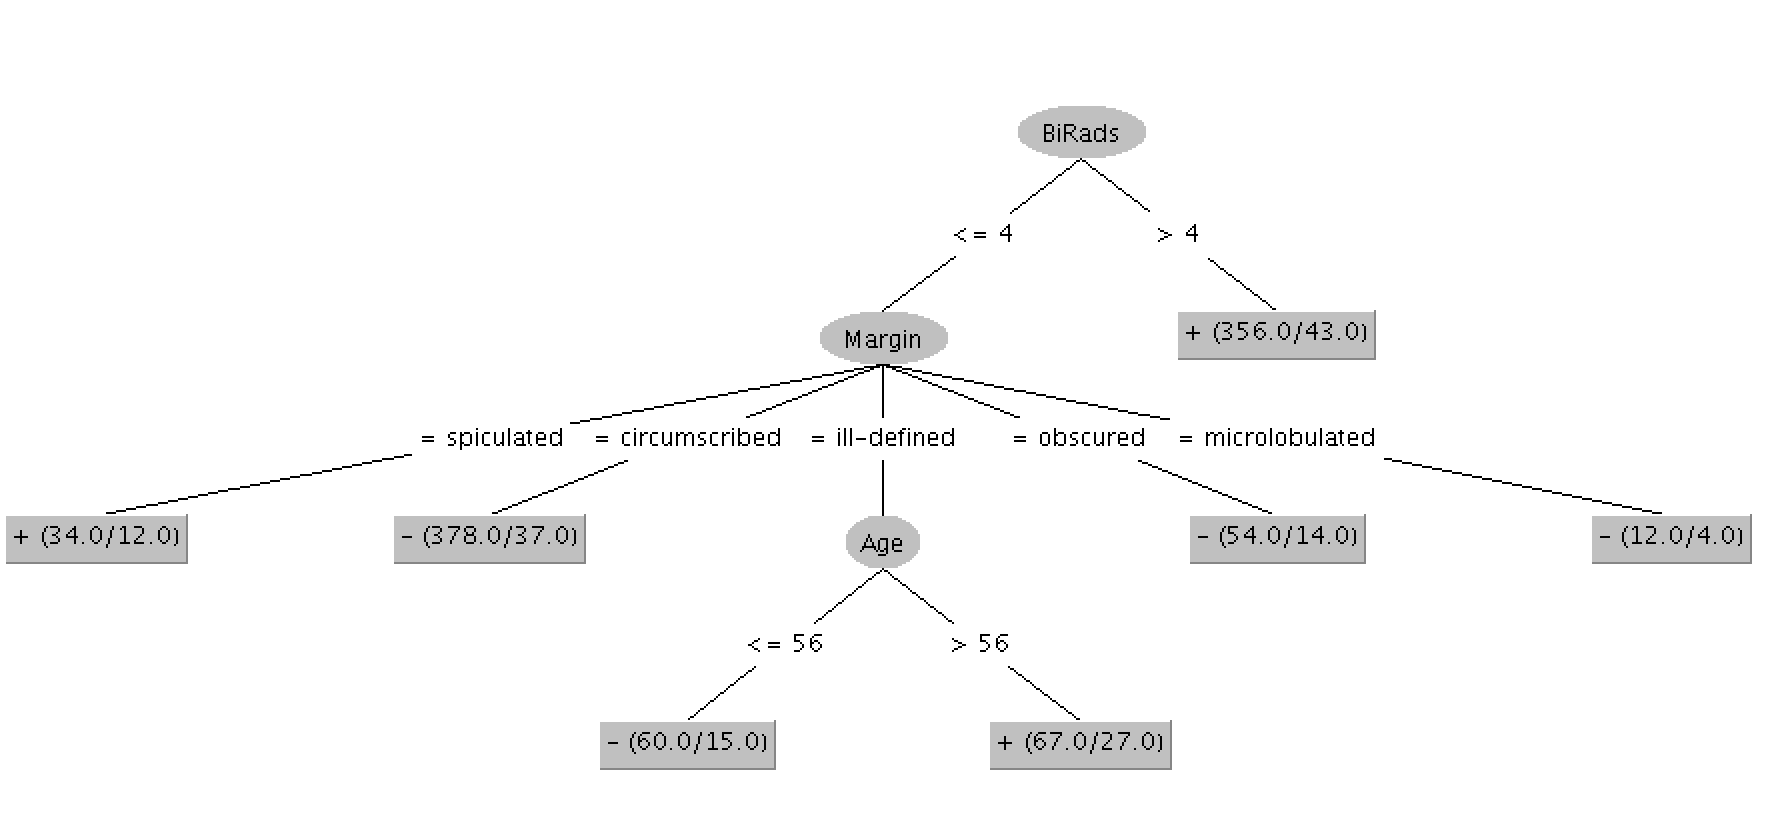
\includegraphics[width=\textwidth]{best-pruned-tree}
      \caption{Best pruned \& highest accuracy decision tree}
      \label{fig:best-pruned-tree}
    \end{figure}

  \subsection{Best Artificial Neural Network}
    As discovered in section \ref{ann-ex} the best structure for an ANN when applied to this dataset is one with two hidden layers. The first layer has 8 neurons and the second has 10, and the optimal learning rate \& momentum are 0.1 and 0.19 respectively with the training time set to 920. The topographical view of the ANN structure described which gives a classification accuracy of 82.86\% can be seen in figure \ref{fig:ann-optimal-structure}.

    \begin{figure}[H]
      \centering
      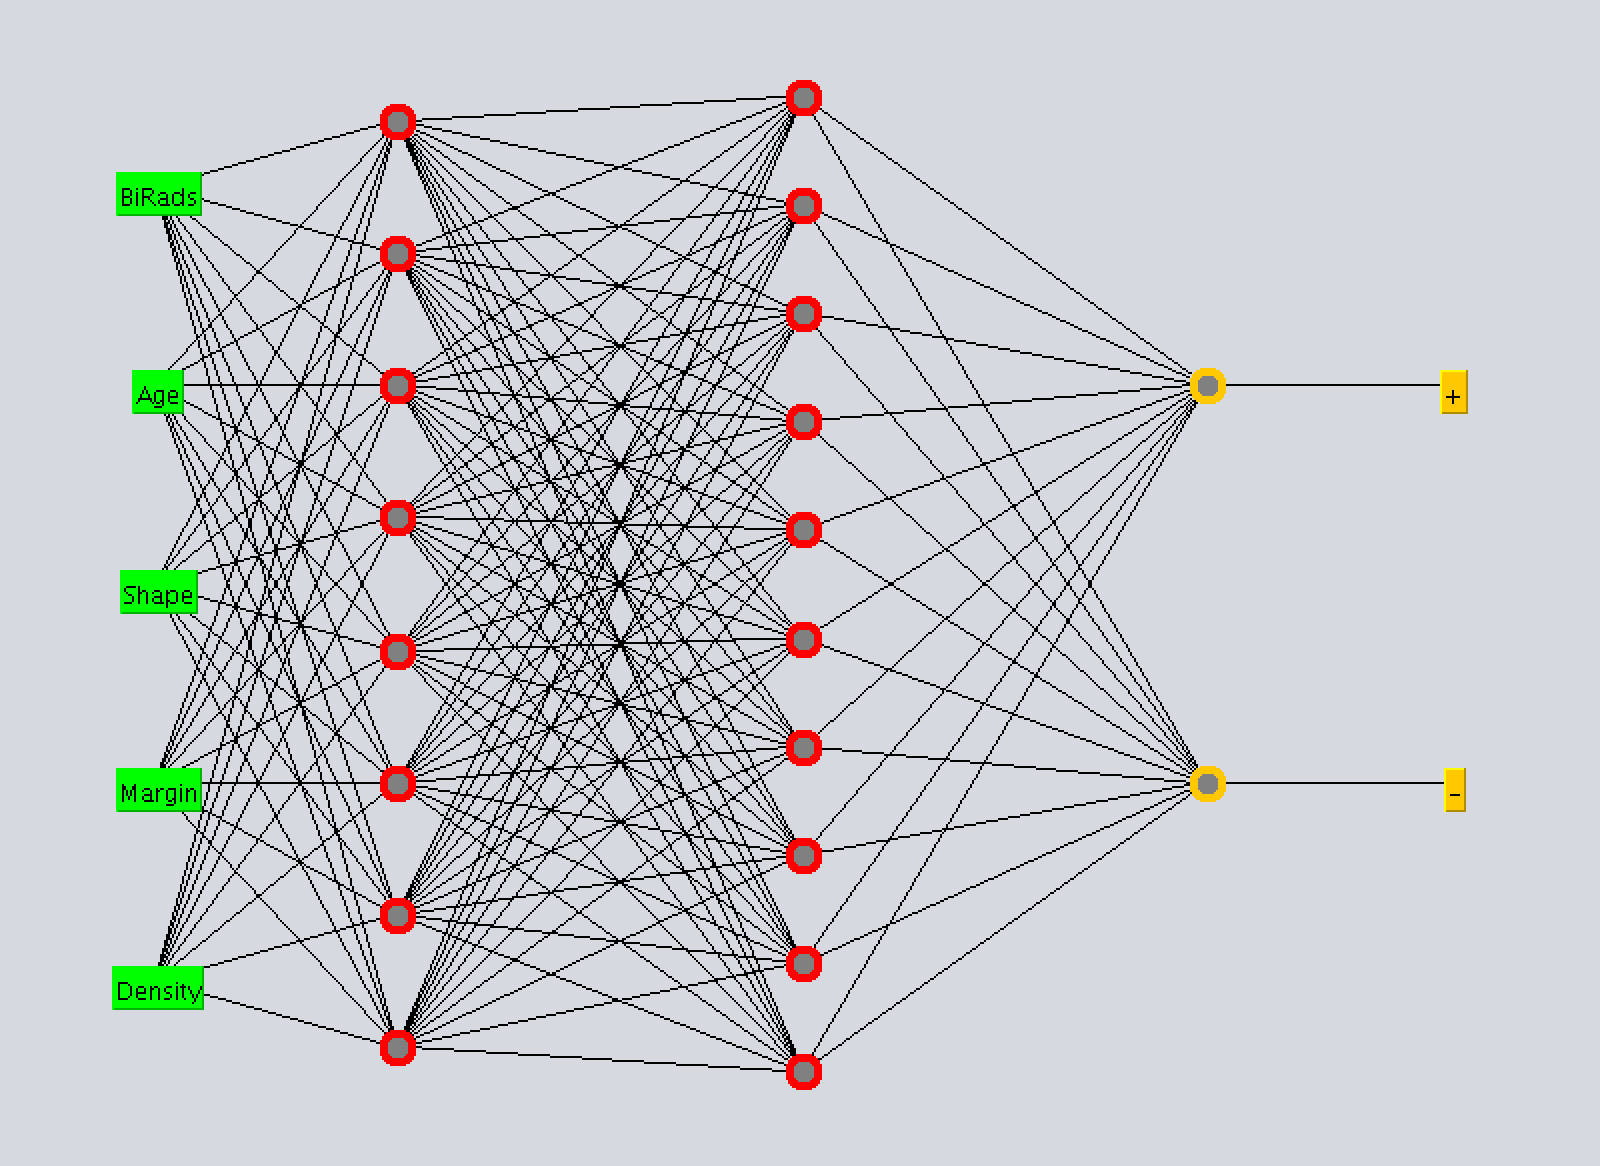
\includegraphics[width=\textwidth]{ann-optimal-structure}
      \caption{Optimal ANN structure}
      \label{fig:ann-optimal-structure}
    \end{figure}

  \subsection{Classifier recommendation}
    The classifier which provided the highest classification accuracy is the J.48 decision tree (see section \ref{dt-execution}), which gave an accuracy score of 83.95\%. Furthermore the decision tree takes much less time to both train and classify therefore it is highly recommended that the client uses the decision tree for the task of classifying mamographical data.

  \subsubsection{Discussion}
    The results displayed in this report highlight that pre-processing steps can increase classification accuracy, for example the highest decision tree accuracy went from 83.84\% to 83.95\%. The Artificial Neural Network did not perform as well for this dataset, even with complex structures. This could be due to the data not being complex enough for an ANN to interpret numerical patterns in the data. On the other hand the decision tree was able to pick out much more simple relationships between attributes with simple tests between them.

\newpage

\bibliographystyle{agsm}
\bibliography{report-jim}

\end{document}
